%%
%% 2016年度 数理統計短期集合研修
%%

\documentclass[11pt,uplatex]{jsarticle}

\usepackage{amsmath}
\usepackage{ascmac}
\usepackage{graphicx}
\usepackage{lmodern}
\usepackage{eclbkbox}
\usepackage{bm}
\usepackage[deluxe]{otf}
\usepackage{listings}
%\usepackage[T1]{fontenc}
%\usepackage{textcomp}
\usepackage{url}
%\usepackage[utf8]{inputenc}

%% ページ番号出力の抑制
\def\thepage{}

%% Listing
\lstset{
  language=,
  basicstyle=\ttfamily\small,
  commentstyle=\texttt,
  classoffset=1,
  keywordstyle=\bfseries,
  frame=single,
  framesep=5pt,
  showstringspaces=false,
  numbers=left,
  stepnumber=1,
  numberstyle=\tiny,
  tabsize=2
}

\begin{document}

\title{ベイジアンMCMCによる統計モデル}
\author{森林総合研究所\\伊東宏樹\footnote{hiroki@affrc.go.jp}}
\date{2016年11月18日}
\maketitle


\section{はじめに}

本講では,理論的な解説については最小限として,
MCMCを使って実際に問題を解くことに主眼を置きたい。
理論面についての解説は末尾の参考文献などを参照されたい。
ソフトウェアとしては,\textsf{R}\cite{R}上にて
\textsf{MCMCpack}\cite{MCMCpack}と
\textsf{JAGS}\cite{JAGS}を使用する
(実習には\textsf{MCMCpack}を使用する)。
また,\textsf{Stan}\cite{Stan}の紹介もおこなう。
\footnote{本テキスト執筆時には,R 3.2.2, MCMCpack 1.3-3, JAGS 3.4.0, Stan 2.8.0を使用した。}

\subsection{MCMCとは?}

MCMCはベイズ推定のための計算手法である。

\paragraph{ベイズ統計}

データ$\bm{x}$が与えられたときの母数(パラメーター)$\bm{\theta}$の
事後確率$\pi(\bm{\theta}|\bm{x})$は,
ベイズの定理により以下のようになる。
\begin{equation}
\pi(\bm{\theta}|\bm{x}) = \frac{f(\bm{x}|\bm{\theta})\pi(\bm{\theta})}
{\int{f(\bm{x}|\bm{\theta})\pi(\bm{\theta})d\bm{\theta}}}\label{bayes1}
\end{equation}
ここで,$f(\bm{x}|\bm{\theta})$は尤度,$\pi(\bm{\theta})$は$\bm{\theta}$の事前確率である。
なお,右辺の分母は定数となるので,
\begin{equation}
\pi(\bm{\theta}|\bm{x}) \propto f(\bm{x}|\bm{\theta})\pi(\bm{\theta})\label{bayes2}
\end{equation}
事後確率は尤度と事前確率との積に比例する。
イメージとしては,事前の知識(事前確率)を,データ(尤度)で更新して,事後確率を得る,
ということになろう。

ここで,母数の事後確率(確率分布としては事後分布)を求めたいわけなのだが,
モデルが複雑な場合は事後確率(事後分布)を解析的に解くことは困難である。
このような問題に対してMCMCは非常に有効である。

%GLMやGLMMの枠組みに収まらないような複雑なモデルもMCMCにより
%解くことができる。

\paragraph{MCMC=MC+MC}

では,そもそも``MCMC''とはなんだろうか?
言葉の面からみると,MCMCは前半のMC (Markov Chain)と後半のMC (Monte Carlo)とに分解できる。

\begin{description}
\item[Markov chain] マルコフ連鎖\\
次の状態$x_{t+1}$が現在の状態$x_{t}$にのみ依存するような確率過程。\\
例:ランダムウォーク。図\ref{random_walk_plot}は,0.5の確率で+1になるか-1になる,というもの。
\end{description}

\begin{figure}[hbtp]
  \begin{center}
    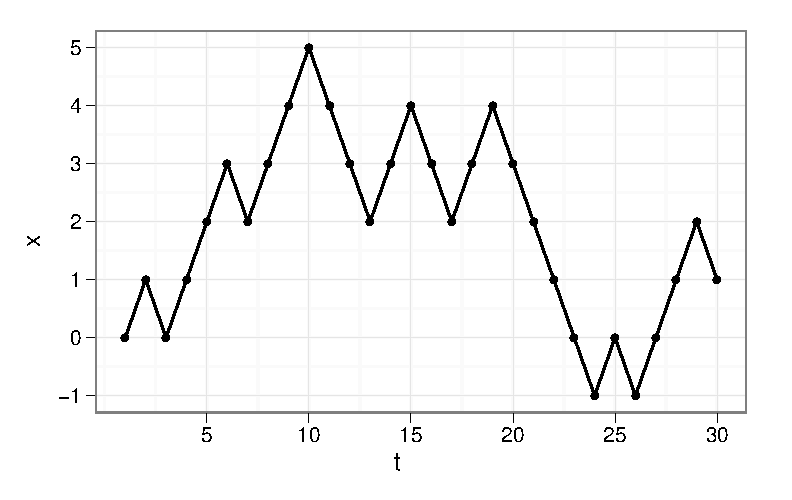
\includegraphics[bb=0 0 380 240, clip, width=300 bp]{random_walk2.pdf}
  \end{center}
  \caption{ランダムウォーク}
  \label{random_walk_plot}
\end{figure}

\begin{description}
\item[Monte Carlo] モンテカルロ(法)\\
乱数を用いた計算アルゴリズムを一般にモンテカルロ法と呼ぶ。
名前は,カジノで有名なモンテカルロ(モナコ)から取られた。
\end{description}

そして,MCMCを一言で説明するなら,

\vspace{2zw}
\hspace{10mm}
\begin{minipage}{110mm}
\begin{breakbox}
\noindent
{\large\bf 乱数を用いてマルコフ連鎖を生成し,それにより母数の事後分布を推定する手法}
\end{breakbox}
\end{minipage}
\vspace{2zw}

\noindent
となるだろう。というのも,

\vspace{2zw}
\hspace{10mm}
\begin{minipage}{110mm}
\begin{breakbox}
\noindent
{\large\bf うまく工夫したマルコフ連鎖をつくってやることにより,
事後分布からのサンプルと見なせる
データをとりだすことができる}
\end{breakbox}
\end{minipage}
\vspace{2zw}

\noindent
からである。

%ページ調整
%\vspace{4zw}

\subsection{MCMCのアルゴリズム}

MCMCのアルゴリズムとしては,Metropolis-Hastingsアルゴリズムや,
その特殊な場合にあたるGibbs samplerがよく用いられる。\cite{PRML,Iba2005,Toyoda,Watanabe}
最近は,Hamiltonian Monte Carlo(またはHybrid Monte Carlo)
\cite{PRML,BDA3,Toyoda2015,Watanabe}
を使用したソフトウェアもある。
アルゴリズムについて詳しく知りたい方は参考文献を参照されたい。
%あとで触れる\textsf{LaplacesDemon}では多数のアルゴリズムが実装されている
%(\ref{LaplacesDemon}節)。

%\subsubsection{Metropolis-Hastingアルゴリズム}
%
%Markov chainにおいて,現在の値$x^{(i)}$の次の値$x^{(i+1)}$を以下のようにして選ぶ。
%
%\begin{enumerate}
%\item $x^{(i+1)}$の候補$y$をある条件付き分布(これをサンプラーと呼ぶ)
%$q(\cdot|\cdot)$にしたがって確率的に決める。
%$y$は$x^{(i)}$を少しだけ動かした値となる。
%\item $y$が,求めたいパラメーターの分布$\pi(\cdot)$に$x^{(i)}$よりもうまく当てはまるなら,
%$x^{(i+1)}$として$y$を採用する。
%$x^{(i)}$の方がうまく当てはまる場合には,その当てはまりやすさに応じて,
%$x^{(i+1)}$として$y$を選ぶか,$x^{(i)}$を選ぶかを確率的に決める。
%その確率$\Pr$は具体的には,
%\begin{equation}
%\Pr = \mathrm{min}\left(1, \frac{\pi(y)q(x^{(i)}|y)}{\pi({x^{(i)}})q(y|x^{(i)})}\right)\label{MH1}
%\end{equation}
%\end{enumerate}
%\noindent
%である。
%なお,ここでminは最小値を返す関数である。
%
%そして,$q(y|x) = q(x|y)$となるようなサンプラーをMetropolis samplerと呼ぶ。
%この場合 式\ref{MH1}は,
%\begin{equation}
%\Pr = \mathrm{min}\left(1, \frac{\pi(y)}{\pi({x^{(i)}})}\right)\label{MH2}
%\end{equation}
%となる。サンプラーとしては正規分布
%\begin{align*}
%q(Y|X) &= \mathrm{Normal}(Y|X, \sigma^2) \notag \\
%  &=\frac{1}{\sqrt{2\pi\sigma^2}}\exp{\left(-\frac{(Y-X)^2}{2\sigma^2}\right)}
%\end{align*}
%が用いられることが多い。
%
%\subsubsection{Gibbs sampler}
%
%Metropolisアルゴリズムの1種だが,必ず採択されるようにサンプラーを工夫してある
%(詳しくは参考文献\cite{Iba2005,Tango,Toyoda}などを参照)。
%%このサンプラーはGibbs samplerと呼ばれる。
%後述(\ref{BUGS}節)のBUGS言語を使用するソフトウェアはこのGibbs samplerを使用できるように
%なっている。
%
%\subsubsection{Hamiltonian Monte Carlo}
%
%変数の移動のアルゴリズムとしてランダムウォークでは効率が悪いので,
%「運動量」をもたせてより効率的に目標分布に収束できるようにしたものである。
%詳細は参考文献\cite{PRML, BDA3, Toyoda2015}を参照されたい。
%後述(\ref{Stan}節)の\textsf{Stan}はこのアルゴリズムを使用している。

\section{MCMCのためのソフトウェア}
\begin{itemize}
\item  \textsf{R}上で: MCMCpackなど
\item 専用ソフトウェア: \textsf{WinBUGS}, \textsf{OpenBUGS}, \textsf{JAGS}, \textsf{Stan}
\begin{itemize}
 \item  \textsf{Stan}以外は,BUGS (\textbf{B}ayesian inference \textbf{U}sing
 \textbf{G}ibbs \textbf{S}ampling)言語\cite{BUGSBook, BUGS}という
 モデリング言語を使用している。
 \label{BUGS}
\item \textsf{Stan}は異なる言語仕様であるが,BUGS言語と似ている。
\item  いずれにも\textsf{R}から使えるようにするパッケージあり。
\end{itemize}
\item \textsf{Python}のパッケージもある(\textsf{PyMC})。
\item 自分でソフトを書く人もいる(C++などで)。
\end{itemize}

\subsection{MCMCpack}

\begin{itemize}
\item ウェブサイト: \texttt{\url{http://mcmcpack.berkeley.edu/}}
\item 最新版: 1.3-4
\item \textsf{R}のパッケージ
\item CRANからインストールできる。
\item Metropolis samplerを使う。
\item \texttt{MCMClogit()},\texttt{MCMCpoisson()}などの関数が用意されており,
これらを使用してMCMC計算ができる。
一部の混合効果モデル(ランダム効果のあるモデル)にも対応している
(\texttt{MCMChregress()},\texttt{MCMChlogit()},
\texttt{MCMChpoisson()}など)。
このように主要なモデルに対応した関数が30個あまりある。
自分で定義した確率分布を使用するときは\texttt{MCMCmetrop1R()}関数を使用する。
参考文献\cite{MCMCpack}に解説あり。
\end{itemize}

%\subsection{LaplacesDemon}
%\label{LaplacesDemon}
%\begin{itemize}
%\item ウェブサイト: \texttt{http://www.bayesian-inference.com/software}
%\item 最新版: 14.06.23
%\item \textsf{R}のパッケージ
%\item CRANには収録されていないので,開発元からソースをダウンロードしてきてインストールする。
%\item さまざまなアルゴリズムを使用できる。
%\item 並列計算にも対応している。
%\end{itemize}


\subsection{WinBUGS}

\begin{itemize}

\item ウェブサイト:\\
  \url{http://www.mrc-bsu.cam.ac.uk/software/bugs/the-bugs-project-winbugs/}
\item 最新版: 1.4.3 (開発は終了している)
\item ソースコードは非公開なので,内部のアルゴリズムの確認や,改造はできない。
\item Windows用ソフトだが,\textsf{Wine}\footnote{\url{http://www.winehq.org/} 名前は,
``Wine Is Not Emulator''の略。なお,\textsf{Wine} 1.2系は\textsf{WinBUGS}と
  非互換なので注意。\textsf{Wine}は,Windows互換レイヤーソフトで,Windows用ソフトウェ
  ア(すべてというわけではない)をWindowsなしで動作させることができる。
  最新の安定版は1.6.2。}を使用
  することで,OS XやLinux,BSDでも使用することが可能。
\item GUI環境はあるがあまり使いやすくない。\textsf{R2WinBUGS}パッケージ
  で \textsf{R}と連携可能なので,そちらから使う方が使いやすい(と思う)。
\end{itemize}

\subsubsection*{インストール}

ウェブサイトからインストーラーをダウンロード
できる。いずれの環境でも\textsf{WinBUGS}のインストール後には1.4.3パッチをあ
て,``key''をインストールすること。``key''をインストールすることにより,
全機能が使えるようになる。

\paragraph{Windowsへのインストール}

インストーラー(\texttt{WinBUGS14.exe})を起動して,あとは指示に従ってい
けばインストールされる。
ただし,Windows Vistaでは,\texttt{C:{\textbackslash}Program~Files}以下に
インストールすると,アクセス制御の
関係でパッチなどが当てられなくなるので,\texttt{C:{\textbackslash}Program~Files}以外への
インストールが推奨されている
\footnote{\url{http://www.mrc-bsu.cam.ac.uk/software/bugs/the-bugs-project-winbugs/#install}}。
インストーラーは64ビットWindowsには非対応である。

\paragraph{OS Xへのインストール}

Macでは,\textsf{Wine}を利用して\textsf{WinBUGS}を使うことができる。
OS Xで\textsf{WinBUGS}を動作させる詳細については,
ネット上の資料
\footnote{\url{http://www001.upp.so-net.ne.jp/ito-hi/stat/winbugs.html}\\
\url{http://nhkuma.blogspot.jp/2012/12/macosx106-107winbugswiner2winbugs.html}\\
\url{http://nhkuma.blogspot.jp/2012/12/macosx108-mountain-lion-winbugs-wine.html}}を参照するとよい。
OS X用の\textsf{Wine.app}\footnote{\url{http://winebottler.kronenberg.org/}}
を利用するか,\textsf{MacPors}\footnote{\url{http://www.macports.org/}}などの
パッケージ管理システムを利用してインストールするのが簡単であろう。

\textsf{Wine}をインストールしたら,
これを使用してWindows用インストーラー
(\texttt{WinBUGS14.exe})を起動
し,\textsf{Wine}環境へ
\textsf{WinBUGS}をインストールする
(デフォルトでは\texttt{\textasciitilde/.wine/drive\_c/Program Files}以下にインストールされる)。


\paragraph{Linuxへのインストール}
\textsf{Wine}を使用する。Ubuntuなどの主要なディストリビューションではパッ
ケージ化されているので,それを利用するとよい(もちろん自分で
コンパイルしてインストールしてもよい)。
\textsf{Wine}を使用してインストー
ラー(\texttt{WinBUGS14.exe})を起動し,\textsf{WinBUGS}をインストールする。

BSDその他UNIXも基本的にはLinuxに準じる。

\subsection{OpenBUGS}

\begin{itemize}
\item ウェブサイト \url{http://www.openbugs.net/}
\item 最新版: 3.2.3
\item オーブンソース(ライセンスはGPL)。しかし開発環境が特
  殊(Black Box Component Builder\footnote{\texttt{http://www.oberon.ch/blackbox.html}}と
  いうものを使用)。
\item WindowsおよびLinuxで動作する。
OS Xでは\textsf{Wine}により利用可能。
\item \textsf{BRUGS}あるいは\textsf{R2OpenBUGS}により
\textsf{R}との連携が可能\cite{Thomas}。
ともにCRANに収録されている。
\end{itemize}

\subsubsection*{インストール}
\paragraph{Windowsへのインストール}
Windows版インストーラーからインストールできる。64ビットWindowsにもインストールできる。
開発元ではWindows XPと8とで動作確認している。

\paragraph{OS Xへのインストール}
\textsf{WinBUGS}と同様に,\textsf{Wine}を導入して,Windows版をインストールする。

\paragraph{Linuxへのインストール}
Linux用ソースパッケージを展開して,コンパイル・インストールする。

%% JAGS
\subsection{JAGS}

\begin{itemize}

\item ウェブサイト:
  \url{http://mcmc-jags.sourceforge.net/}
  
\item 作者ブログ:
  \url{http://martynplummer.wordpress.com/}  

\item 最新版: 4.0.0

\item オープンソース(ライセンスはGPL)。再配布はもちろん,内部の解析,改
  造なども自由にできる。CおよびC++で書かれていて一般的な開発環境でコンパイル
  可能\footnote{農林水産研究情報総合センターの科学技術計算システム2012でも自分
  でコンパイルして利用できた。}
  (ただし,BLASやLAPACKといった数値演算ライブラリは必要)。

\item コマンドラインからの操作となるが,\textsf{rjags}や\textsf{R2jags},\textsf{runjags}
といったパッケージを
利用することで,\textsf{R}から使用することも可能。
いずれもCRANに収録されている。

\item \textsf{WinBUGS}で解析できる一部のモデルは解析できない
  \footnote{\url{http://hosho.ees.hokudai.ac.jp/~kubo/ce/JagsMisc.html}}。
 もっとも,\textsf{WinBUGS}よりも柔軟なところもある
  \footnote{\url{http://ito-hi.blog.so-net.ne.jp/2007-02-01-1}}。
  
\item \textsf{OpenBUGS}を実行速度を比較すると,いくつかのモデルではとくに遅いことがあるものの,
平均的にはだいたい同等といったところであると
いう\footnote{\url{http://martynplummer.wordpress.com/2010/09/20/how-fast-is-jags/}}。

\end{itemize}

\subsubsection*{インストール}
WindowsおよびOS Xにはインストーラーが用意されている。
Linux版主要ディストリビューションにはバイナリパッケージがあるので
それを利用できる。
開発環境があれば,ソースから自分でコンパイルすることも比較的簡単である。
詳細はインストールマニュアルを参照。

%% Stan
\subsection{Stan}
\label{Stan}
\begin{itemize}

\item ウェブサイト:
  \url{http://mc-stan.org/}

\item 最新版: 2.8.0
\item オープンソース(BSDライセンスまたはGPL3)。再配布,内部の解析,改
  造なども自由にできる。
\item \textsf{RStan}という\textsf{R}のパッケージもあり,CRANに収録されている。
また,Pyhtonインターフェイスの\textsf{PyStan}もある。
コマンドラインから実行するものは\textsf{CmdStan}と呼ばれる。
\item Stan $\rightarrow$ C++ $\rightarrow$ ネイティブバイナリ,とコンパイルして実行する。
ネイティブバイナリとして実行されるので,インタプリタ形式と比較して高速である。
\item OS X, Windows, Linuxなどに対応している。
\item Hamiltonian Monte Carlo法\cite{PRML, BDA3, Toyoda2015}を使用し,
通常のMCMCよりも高速に目的分布に収束する。
\item 言語仕様は,BUGSと似てはいるが,異なる。
\end{itemize}

\subsubsection*{インストール}
RStanはCRANからインストール可能。
CmdStanのインストールには開発環境(C++など)が必要となる。
詳細はウェブサイトやマニュアルを参照。


\pagebreak

%%
%% ここから実演
%%
\section{実例}

ここからは,簡単な実例を通してMCMCの使い方をみていきたい。

\subsection{最初のモデル: ポアソン回帰}

%簡単な例題から。
まずは次の例題をMCMCを使って解いてみる。

\vspace{1zw}

\hspace{18mm}
\begin{minipage}{100mm}
\begin{breakbox}
ポアソン分布することがわかっている ある母集団から,\\
\hspace{10mm} $\bm{x} = (3, 1, 4, 3, 3, 6, 4, 1, 6, 4, 
       1, 7, 4, 4, 1, 4, 0, 3, 9, 4)$\\
という標本が得られたとき,その母平均$\lambda$を推定する。
\end{breakbox}
\end{minipage}

\vspace{1zw}

\subsubsection{MCMCpoisson()による例}

まずここでは \textsf{R}上で,\textsf{MCMCpack}パッケージの\textsf{MCMCpoisson()}関数
を使用してポアソン回帰をおこなう。
\textsf{R}スクリプトは,サンプルファイルの\texttt{example1.R}である。
\vspace{1zw}

まずは,\textsf{MCMCpack}パッケージを呼び出す。
(以下,実行例をボックスの中にしめす。なお,``\texttt{>}''は入力行のプロンプトを,
``\texttt{+}''は,前の行からの継続をそれぞれ示す記号であり,実際には入力不要。)

%%\begin{breakbox}
\begin{lstlisting}
> library(MCMCpack)
\end{lstlisting}
%\end{breakbox}
%
結果を収納するために,\texttt{post1}という要素数3のリストを作成する。

\begin{lstlisting}
> post1 <- vector("list", 3)
\end{lstlisting}
%
つづいて,\texttt{MCMCpoisson()}を実行する。
\texttt{MCMCpoisson()}では,
$\log(\lambda)$が推定される。

実際に推定をする前に,まずはMCMCの挙動をみるために最初の部分の軌跡を
くわしくみてみることにする。
\begin{lstlisting}
> post1[[1]] <- MCMCpoisson(x ~ 1, beta.start = 1,
+                           burnin = 0, mcmc = 400,
+                           thin = 1,
+                           tune = 0.8, seed = 1117,
+                           verbose = 20)
\end{lstlisting}
%\noindent
引数の説明をする。
\texttt{x $\sim$ 1}はモデル式(\texttt{glm()}などと同様)である。
モデル式の右側は``1''だけなので,これはつまり
\begin{align*}
\bm{X} &\sim \mathrm{Poisson}(\lambda)
%\hspace{1zw}{\text あるいは}\hspace{1zw}
%\Pr(\bm{X}|\lambda) = \mathrm{Poisson}(\bm{X}|\lambda)
\\
\log\lambda &= C
\end{align*}
で,$C$を推定するということになる。
なお,このときの事前分布は実質的には存在しないものとして扱われている
\footnote{事前分布を指定するときは,\texttt{b0}引数(平均)と
\texttt{B0}引数(精度:分散の逆数)を使う。}
(improperな無情報事前分布。詳細は後述)。

\texttt{beta.start}はパラメーター(ここでは$\log\lambda$)の初期値,
\texttt{burnin}は初期値に依存しているおそれがあるので捨てる部分である
(burn-in期間。この例では0としている。詳しくは後述)。
\texttt{mcmc}はサンプルを得る繰り返し回数,
\texttt{thin}はサンプルを得る間隔(この例では1,すなわち毎回サンプルを得るようにしている
\footnote{サンプル間の自己相関が強いモデルではこの間隔を空ける。
ただし,thinningはよく考えられず使われているという指摘もある\cite{Link2012}。}),
\texttt{tune}はランダムウォークの大きさにかかわるパラメーター,
\texttt{seed}は疑似乱数のタネである。これを指定することにより乱数系列が固定され,
あとで同じ計算をさせたときに結果が同じになる。
\texttt{verbose}は途中経過を表示する間隔。ここでは,20回ごとに途中経過を表示するように
している。

まずはMarkov chainの軌跡をプロットする。結果は図\ref{MCMCpoisson_plot}。

\begin{lstlisting}
> plot(post1[[1]], density = FALSE, col = 1, las = 1)
\end{lstlisting}
%
\begin{figure}[hbtp]
  \begin{center}
    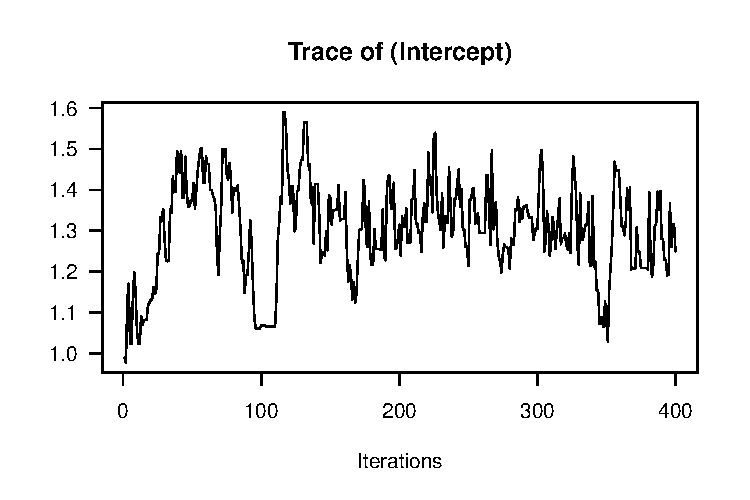
\includegraphics[bb=0 0 360 240, clip, width=240 bp]{example1-1.pdf}
  \end{center}
  \caption{\texttt{MCMCpoissonR()}によるMarkov chainの軌跡}
  \label{MCMCpoisson_plot}
\end{figure}

最初から50回目くらいまでは,初期値の影響が残っていることがわかる。
すくなくとも この部分はburn-in期間として除外する必要がある。

\texttt{tune}の値を変えると収束の速度が変わる。
小さすぎると,収束が遅くなる。
かといって,大きすぎても採択率が悪くなりすぎて,やはりなかなか収束しなくなる。
採択率の目安は(どんな場合にでもあてはまるわけではないが)1〜2次元のモデルで0.5,
高次のモデルでは0.25とされている\cite{IMCMR}。

%ページ調整
\vspace{4zw}


乱数系列と初期値を変えて同様の計算を繰り返してみる。

\begin{lstlisting}
> post1[[2]] <- MCMCpoisson(x ~ 1, beta.start = 5,
+                           burnin = 0, mcmc = 400, thin = 1,
+                           tune = 0.8, seed = 1123,
+                           verbose = 20)
> post1[[3]] <- MCMCpoisson(x ~ 1, beta.start = 10,
+                           burnin = 0, mcmc = 400, thin = 1,
+                           tune = 0.8, seed = 1129,
+                           verbose = 20)
\end{lstlisting}
%
結果を\texttt{mcmc.list}形式に変換して,軌跡をプロットする。
結果は図\ref{MCMC3}。

\begin{lstlisting}
> post1.mcmc <- mcmc.list(post1)
> plot(post1.mcmc, density = FALSE, ylim = c(0, 10), las = 1)
\end{lstlisting}
%

\begin{figure}[hbtp]
  \begin{center}
    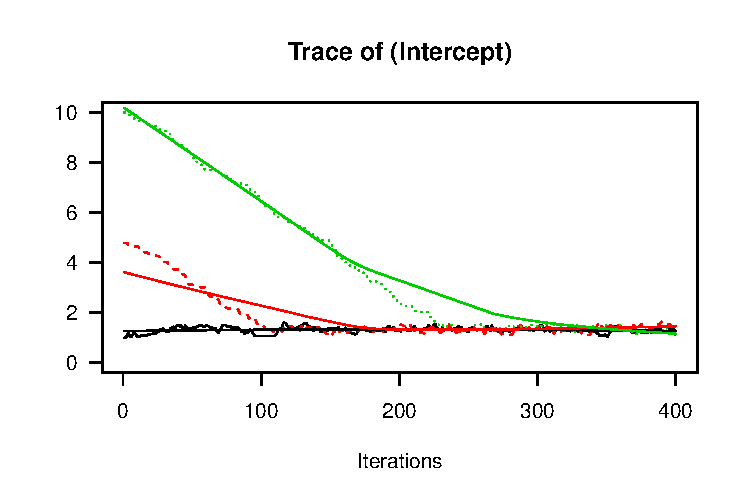
\includegraphics[bb=0 0 360 240, clip, width=260 bp]{example1-2.pdf}
  \end{center}
  \caption{Markov chainを3つにした結果}
  \label{MCMC3}
\end{figure}\noindent
初期値により,その影響の残る期間は変わるが,同じような値に
収束しているように見える。

では次に,実際に事後分布のサンプルを得ることとする。
burn-inを500回,burn-in後の繰り返し回数を1000回,
サンプル取得間隔を1回(つまり毎回),
Markov chainの数は3とする。
このとき,取得されるサンプルの大きさは$1000\div1\times3=3000$となる。

\begin{lstlisting}
> post2 <- vector("list", 3)
> burnin <- 500
> mcmc <- 1000
> thin <- 1
> tune <- 2
> verbose = 0
> post2[[1]] <- MCMCpoisson(x ~ 1, beta.start = 1,
+                           burnin = burnin, mcmc = mcmc,
+                           thin = thin,
+                           tune = tune, seed = 1117,
+                           verbose = verbose)
> post2[[2]] <- MCMCpoisson(x ~ 1, beta.start = 5,
+                           burnin = burnin, mcmc = mcmc,
+                           thin = thin,
+                           tune = tune, seed = 1123,
+                           verbose = verbose)
> post2[[3]] <- MCMCpoisson(x ~ 1, beta.start = 10,
+                           burnin = burnin, mcmc = mcmc,
+                           thin = thin,
+                           tune = tune, seed = 1129,
+                           verbose = verbose)
> post2.mcmc <- mcmc.list(post2)
> 
> plot(post2.mcmc)
\end{lstlisting}

結果を図示する(図\ref{MCMC_plot})。
\begin{lstlisting}
> plot(post2.mcmc)
\end{lstlisting}

\begin{figure}[hbtp]
  \begin{center}
    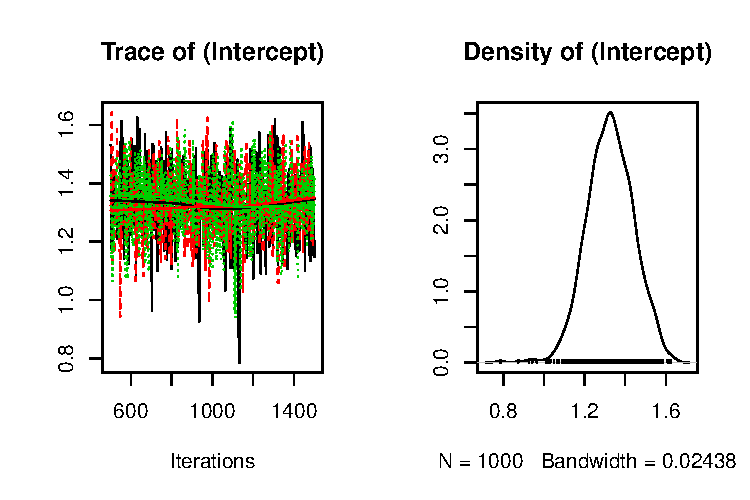
\includegraphics[bb=0 0 360 240, clip, width=260 bp]{example1-3.pdf}
  \end{center}
  \caption{Markov chainをの軌跡と,$\lambda$の事後分布}
  \label{MCMC_plot}
\end{figure}

要約を表示する。
\begin{lstlisting}
> summary(post2.mcmc)

Iterations = 501:1500
Thinning interval = 1 
Number of chains = 3 
Sample size per chain = 1000 

1. Empirical mean and standard deviation for each variable,
   plus standard error of the mean:

          Mean             SD       Naive SE Time-series SE 
      1.327263       0.114073       0.002083       0.004269 

2. Quantiles for each variable:

 2.5%   25%   50%   75% 97.5% 
1.109 1.251 1.327 1.406 1.548 

\end{lstlisting}
%
ベイズ推定ではパラメーターの推定値も確率的に(つまり事後分布として)与えられる。
その代表値としては一般に平均や中央値が用いられる。
また,95\%信用区間\footnote{「頻度主義」統計における信頼区間とは実は違うもの}も同時に使われることが多い。
この例では,
$\log\lambda$の事後分布の平均値(事後平均)が1.33,95\%信用区間が
1.11〜1.55と推定された。事後平均に対応する$\lambda$の値は$\exp(1.33)=3.78$と
いうことになる。

\subsubsection{MCMCmetrop1R()による例}

つぎに,一般的なベイズモデリングが可能な\texttt{MCMCmetrop1R()}を
同じデータに適用した例をしめす。
\texttt{MCMCpoisson()}はポアソン回帰専用だが,
\texttt{MCMCmetrop1R()}はより自由なモデリングが可能である。

まず,サンプリングをおこなうための関数を定義する。
ここでは,事前分布$\times$尤度の対数を返り値としている。
この関数をあとで\texttt{MCMCmetrop1R()}に引数のひとつとして与えてやる。
\begin{lstlisting}
> LogPoisFun <- function(lambda, x) {
+   # Poisson distribution: p(x) = lambda^x exp(-lambda)/x!
+   if (lambda >= 0) {    # lambda must be non-negative
+     # prior: dunif(0, 10^4)
+     log(ifelse(lambda >= 0 & lambda < 10^4, 10^-4, 0)) + 
+       # log likelihood
+       sum(log(lambda^x * exp(-lambda) / factorial(x)))
+   } else {
+     -Inf
+   }
+ }
\end{lstlisting}

ここでは,$\lambda$の事前分布は,0〜$10^{4}$の一様分布
としている。
\begin{align*}
\lambda &\sim \mathrm{Uniform}(0, 10^{4}) \\
\intertext{すなわち}
\mathrm{Pr}(\lambda) &=
\begin{cases}
10^{-4} & 0 \leq \lambda  < 10^{4} \\
0 & 上以外の場合 \\
\end{cases}
%\label{noninformative}
\end{align*}
事前分布として与えるべき確率分布があらかじめわからない場合には
このような幅が広く,とくに意味のない分布が与えられることが多い。
このような事前分布を「無情報事前分布」という。
一様分布のほか,分散の大きい正規分布やガンマ分布もよく用いられる。
また,この前の例のように実質的には存在しないと扱われる
($(-\infty, \infty)$の一様分布)こともある。
このような事前分布は,
improper priorと呼ばれる。

ポアソン分布の確率密度関数が$f(x)=\lambda^{x}e^{-\lambda}/x!$なので,
パラメーター$\lambda$のもとでデータ$\bm{X}$が得られる
尤度$L(\bm{X}|\lambda)$は以下の式\ref{likelihood_pois}になる。
\begin{align}
L(\bm{X}|\lambda) = \prod_{i = 1}^{N}\frac{\lambda^{X_{i}}e^{-\lambda}}{X_{i}!}
\label{likelihood_pois}
\end{align}

したがって,事後分布は以下のようになる。
\begin{align}
\Pr(\lambda|\bm{X}) &\propto L(\bm{X}|\lambda) \mathrm{Pr}(\lambda) \\
L(\bm{X}|\lambda) \mathrm{Pr}(\lambda) &=\begin{cases}
 \prod_{i = 1}^{N}\frac{\lambda^{X_{i}}e^{-\lambda}}{X_{i}!} \times 10^{-4} & 0 \leq \lambda  < 10^{4}  \\
 0 & 上以外の場合  \label{posterior} \\
\end{cases}
\end{align}

\noindent
上の \textsf{R}関数\texttt{LogPoisFun()}では式\ref{posterior}を対数和として計算している。
%\begin{align*}
%\log\mathrm{Pr}(\lambda|\bm{X}) &= \sum_{i = 1}^{N}\log\frac{\lambda^{X_{i}}e^{-\lambda}}{X_{i}!} + \log10^{-4} \\
%\end{align*}

つづいて,\texttt{MCMCmetrop1R()}を実行する。
引数\texttt{fun}は,サンプリングをおこなう事後分布の関数
(詳細は\texttt{help(MCMCmetrop1R)}を参照)で,
先に定義した\texttt{LogPoisFun}を与えている。
その他の引数は\texttt{MCMCpoisoon()}におなじである。
ここでも3本のMarkov chainを計算させているが,\texttt{lapply()}関数を使って
プログラムを短くしている。

\vspace{1zw}
\begin{lstlisting}
> chains <- 1:3
> inits <- c(1, 10, 20)
> seeds <- c(1117, 1123, 1129)
> post3 <- lapply(chains,
+                 function(chain) {
+                   MCMCmetrop1R(fun = LogPoisFun,
+                                theta.init = inits[chain],
+                                burnin = 1000, mcmc = 1000,
+                                thin = 1,
+                                tune = 2, seed = seeds[chain],
+                                verbose = 0, logfun = TRUE,
+                                x = x)
+                 })


@@@@@@@@@@@@@@@@@@@@@@@@@@@@@@@@@@@@@@@@@@@@@@@@@@@@@@@@@
The Metropolis acceptance rate was 0.49600
@@@@@@@@@@@@@@@@@@@@@@@@@@@@@@@@@@@@@@@@@@@@@@@@@@@@@@@@@


@@@@@@@@@@@@@@@@@@@@@@@@@@@@@@@@@@@@@@@@@@@@@@@@@@@@@@@@@
The Metropolis acceptance rate was 0.48850
@@@@@@@@@@@@@@@@@@@@@@@@@@@@@@@@@@@@@@@@@@@@@@@@@@@@@@@@@


@@@@@@@@@@@@@@@@@@@@@@@@@@@@@@@@@@@@@@@@@@@@@@@@@@@@@@@@@
The Metropolis acceptance rate was 0.51000
@@@@@@@@@@@@@@@@@@@@@@@@@@@@@@@@@@@@@@@@@@@@@@@@@@@@@@@@@
\end{lstlisting}

\vspace{1zw}

結果の要約を表示する。
\begin{lstlisting}
> summary(post3.mcmc)

Iterations = 1001:2000
Thinning interval = 1 
Number of chains = 3 
Sample size per chain = 1000 

1. Empirical mean and standard deviation for each variable,
   plus standard error of the mean:

          Mean             SD       Naive SE Time-series SE 
      3.823640       0.435003       0.007942       0.016180 

2. Quantiles for each variable:

 2.5%   25%   50%   75% 97.5% 
3.059 3.529 3.801 4.085 4.744 

\end{lstlisting}

\vspace{1zw}

\paragraph{収束診断}
この例ではうまく収束したが,いつでもうまくいくというものでもない。
うまく収束しなかった例を図\ref{bad_mcmc}にしめす。
\begin{figure}[htbp]
	\begin{center}
		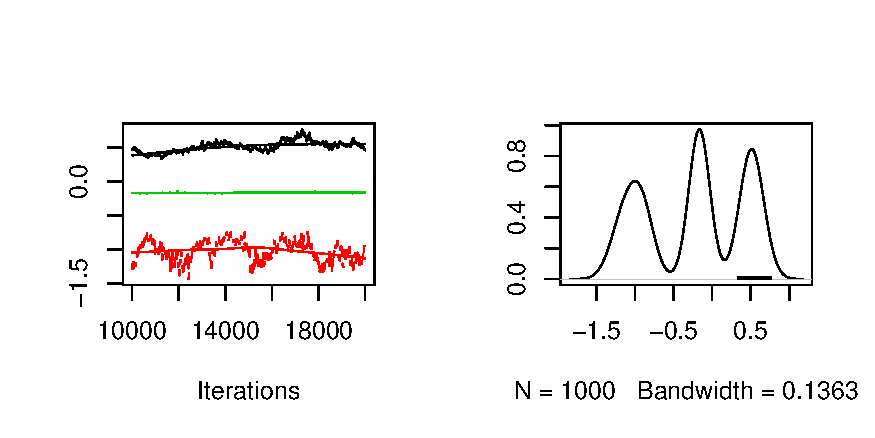
\includegraphics[bb=0 0 420 210, clip, width=320 bp]{bad_mcmc.pdf}
	\end{center}
	\caption{うまく収束しなかった場合}
	\label{bad_mcmc}
\end{figure}

収束状況の診断のためには,Gelman-Rubinの収束診断($\Hat{R}$; Rhat)がよく使われる。
\textsf{R}では,\texttt{coda}パッケージの\texttt{gelman.diag()}関数などで計算できる。
収束していればこの値が1に近くなる(この計算のためには複数のchainが必要である)。
詳細は\texttt{help(gelman.diag)}などを参照されたい。
$\Hat{R}$の値は一般には1.1以下でよいとされるが,必ず軌跡とあわせ見て,
収束しているかどうか判断するべきである。


%ページ調整
\pagebreak
\begin{lstlisting}
> gelman.diag(post3.mcmc)
Potential scale reduction factors:

     Point est. Upper C.I.
[1,]          1       1.01

\end{lstlisting}

\vspace{1zw}

マルコフ連鎖が1本のときにも使える方法としてはGewekeの収束診断
(\texttt{coda}パッケージでは\texttt{geweke.diag()}関数)がある。
マルコフ連鎖の最初の部分と後半との差をZ値であらわす。
$|Z|>1.96$のとき危険率5\%で差がある(定常状態に達していない)ことになる。
詳細は\texttt{help(geweke.diag)}などを参照。
\begin{lstlisting}
> geweke.diag(post3.mcmc)
[[1]]

Fraction in 1st window = 0.1
Fraction in 2nd window = 0.5 

   var1 
0.05941 


[[2]]

Fraction in 1st window = 0.1
Fraction in 2nd window = 0.5 

  var1 
-1.898 


[[3]]

Fraction in 1st window = 0.1
Fraction in 2nd window = 0.5 

  var1 
0.9038 


\end{lstlisting}

\texttt{coda}パッケージの関数のほか,\texttt{boa} (Bayesian Output Analysis)という
パッケージでも収束診断やプロットをおこなうことができる。

%ページ調整
%\pagebreak


%%
%% ロジスティック回帰
%%
\subsection{ロジスティック回帰}
\label{logistic}


つぎに,以下の問題をMCMCを使用して解いてみる。
\vspace{1zw}

\hspace{18mm}
\begin{minipage}{100mm}
\begin{breakbox}
\noindent
ある生物の集団があったとする。
ある薬品がその生物に及ぼす効果を調べるために,
$N$(=11)段階($\bm{x} = (0, 1, 2, 3, 4, 5, 6, 7, 8, 9, 10)$単位)に薬品の量を変えて
その生物への投与試験をおこなった。
それぞれの量を$K$(=10)個体ずつに
与えたところ,その量$\bm{x}$に応じて
10個体中$\bm{y} = (1, 2, 2, 6, 4, 5, 8, 9, 9, 9, 10)$個体が死亡したとする。
このとき,$\bm{x}$と$\bm{y}$との関係をモデル化し,パラメーターを推定する。
\end{breakbox}
\end{minipage}
\vspace{1zw}

$\bm{x}$と$\bm{y}$との関係をプロットしてみると,図\ref{example2_plot}の
ようになる。

\begin{figure}[htbp]
  \begin{center}
    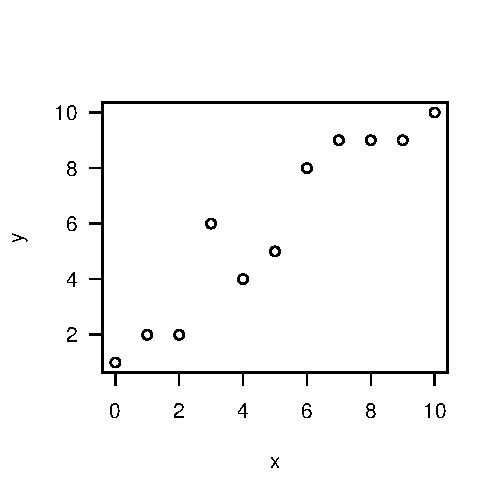
\includegraphics[bb=0 0 240 240, clip, width=160 bp]{example2.pdf}
  \end{center}
  \caption{\ref{logistic}で使用するデータ}
  \label{example2_plot}
\end{figure}


\subsubsection{MCMCpackによる例}

まず,\textsf{MCMCpack}で解いてみる。
\textsf{R}スクリプトは\texttt{example2.R}。

\textsf{MCMCpackage}を読み込む。
\begin{lstlisting}
> library(MCMCpack)
\end{lstlisting}

\paragraph{データ}
データを用意する。
\texttt{data}データフレームの\texttt{y}要素には,各試行ごとの
生死(生=0, 死=1)の結果を入れるようにしている。
\begin{lstlisting}
> x <- c(0, 1, 2, 3, 4, 5, 6, 7, 8, 9, 10)
> y <- c(1, 2, 2, 6, 4, 5, 8, 9, 9, 9, 10)
> k <- 10
> data <- data.frame(x = rep(x, each = k),
+                    y = c(sapply(y, function(i)
+                                      c(rep(0, k - i), rep(1, i)))))
\end{lstlisting}

\paragraph{モデルとあてはめ}
\texttt{y $\sim$ x}をモデル式として,\texttt{MCMClogit()}関数によりベイズ推定をおこなう。
\texttt{MCMClogit()}関数はロジスティック回帰をおこなう\textsf{MCMCpack}の関数。
以下の例ではchainの数を3,burn-inの回数を2000,burn-in後の繰り返し回数を2,
サンプリング間隔を2としている。
\begin{lstlisting}
> chains <- 1:3
> inits <- c(1, 10, 20)
> seeds <- c(12, 123, 1234)
> post <- lapply(chains,
+                function(chain) {
+                  MCMClogit(y ~ x,
+                            data = data,
+                            burnin = 2000, mcmc = 2000,
+                            thin = 2,
+                            tune = 1.1, verbose = 500,
+                            seed = seeds[chain])
+                 })


MCMClogit iteration 1 of 4000 
beta = 
  -2.51563
   0.57885
Metropolis acceptance rate for beta = 1.00000

        :
        :
        
MCMClogit iteration 3501 of 4000 
beta = 
  -2.23947
   0.53340
Metropolis acceptance rate for beta = 0.52699



@@@@@@@@@@@@@@@@@@@@@@@@@@@@@@@@@@@@@@@@@@@@@@@@@@@@@@@@
The Metropolis acceptance rate for beta was 0.52400
@@@@@@@@@@@@@@@@@@@@@@@@@@@@@@@@@@@@@@@@@@@@@@@@@@@@@@@@
\end{lstlisting}

結果を\texttt{mcmc.list}形式に変換して,
軌跡と事後分布を表示する(図\ref{plot_coda_mcmcpack})。
\begin{lstlisting}
> post.mcmc <- mcmc.list(post)
> plot(post.mcmc)
\end{lstlisting}


\begin{figure}[htbp]
	\begin{center}
		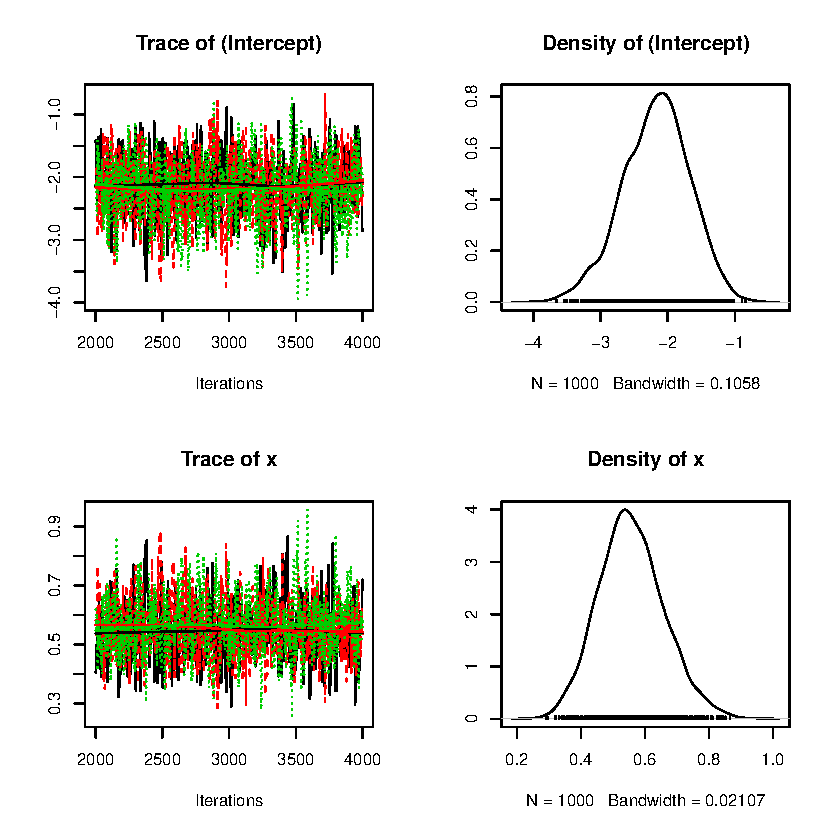
\includegraphics[bb=0 0 400 400, clip, width=300 bp]{example2_results.pdf}
	\end{center}
	\caption{\textsf{coda}クラスオブジェクトのplot出力(MCMCpack)}
	\label{plot_coda_mcmcpack}
\end{figure}

%ページ調整
\vspace{3zw}

収束診断のため,Gelman-Rubin統計量(\^R)を表示する。
\begin{lstlisting}
> gelman.diag(post.mcmc)
Potential scale reduction factors:

            Point est. Upper C.I.
(Intercept)       1.00       1.02
x                 1.01       1.02

Multivariate psrf

1.01
\end{lstlisting}
図\ref{plot_coda_mcmcpack}の結果と合わせ,うまく収束していると
判断できる。

結果を表示する。
\begin{lstlisting}
> summary(post.mcmc)

Iterations = 2001:3999
Thinning interval = 2 
Number of chains = 3 
Sample size per chain = 1000 

1. Empirical mean and standard deviation for each variable,
   plus standard error of the mean:

               Mean     SD Naive SE Time-series SE
(Intercept) -2.1738 0.4948 0.009034        0.01891
x            0.5575 0.1016 0.001856        0.00403

2. Quantiles for each variable:

               2.5%     25%     50%     75%   97.5%
(Intercept) -3.2003 -2.5160 -2.1490 -1.8405 -1.2595
x            0.3675  0.4883  0.5518  0.6204  0.7736

\end{lstlisting}
切片の事後平均が-2.17,95\%信用区間が-3.20〜-1.26,
xの係数の事後平均が0.56,95\%信用区間が0.37〜0.77と推定された。


\subsubsection{JAGSによる例}

つづいて,同じデータを\textsf{JAGS}でベイズ推定する。
\textsf{R}スクリプトは\texttt{example2\_JAGS.R}。

%\paragraph{JAGSを使うための設定}

\textsf{R}で\textsf{JAGS}を使用するため,
\textsf{rjags}パッケージを呼び出す。
%あらかじめ,\textsf{R2OpenBUGS}パッケージをインストール
%しておくこと。
\begin{lstlisting}
> library(rjags)
\end{lstlisting}

\paragraph{データ}
\textsf{R}上で下のようにデータを用意する。
\begin{lstlisting}
> k <- 10
> x <- c(0, 1, 2, 3, 4, 5, 6, 7, 8, 9, 10)
> y <- c(1, 2, 2, 6, 4, 5, 8, 9, 9, 9, 10)
> n <- length(x)
\end{lstlisting}

%ページ調整
%\pagebreak

\paragraph{モデル}
モデルは,BUGS言語で記述したものをファイル(この例では
``\texttt{example2\_model.txt}''という
ファイル名)に保存しておく。
内容は以下のようなものである。
\texttt{MCMCpack}パッケージの\texttt{MCMClogit()}関数でのモデル記述にくらべると
複雑だが,これはさまざまなモデルを記述できる汎用性のためである。

\begin{lstlisting}
model {
  for (i in 1:N) {
    Y[i] ~ dbin(p[i], K)
    logit(p[i]) <- beta + beta.x * X[i]
  }
  beta ~ dnorm(0, 1.0E-6)
  beta.x ~ dnorm(0, 1.0E-6)
}
\end{lstlisting}


では,このモデルについて詳しくみてみよう。
%\begin{minipage}{110mm}
%\begin{lstlisting}
%  for (i in 1:N) {
%    Y[i] ~ dbin(p[i], K)
%    logit(p[i]) <- beta + beta.x * X[i]
%  }
%\end{lstlisting}
%\end{minipage}
%\noindent
2行目から5行目がこの部分がモデルの中心部である。
\texttt{for}ループの構文で,\texttt{for}ブロック内の式の変数\texttt{X[i]}, \texttt{Y[i]}, 
\texttt{p[i]}の\texttt{i}の範囲が
$i \in 1, 2, \dots, N$であることを示している。
\texttt{dbin(p, n)}は二項分布$\mathrm{Binomial}(n, p)$
(\texttt{p}は確率。\texttt{n}は試行回数)。
``\texttt{\textasciitilde}''(チルダ)は,左辺の変数が右辺の確率分布に従うことをしめす。
\texttt{logit(p)}はロジット関数
$\mathrm{logit}(p) = \log(p/(1-p))$
である。
ここでは,\texttt{Y}が,試行回数\texttt{K}および確率\texttt{p}の二項分布に
従い,\texttt{p}のロジットが\texttt{X}と線形の関係にあるとモデル化している。
%なお,行末の``;''はなくてもよい。

つぎに,6行目から7行目で\texttt{beta}および\texttt{beta.x}の事前分布を定義している。
%\begin{minipage}{110mm}
%\begin{lstlisting}
%  beta ~ dnorm(0.0, 1.0E-6);
%  beta.x ~ dnorm(0.0, 1.0E-6);
%\end{lstlisting}
%\end{minipage}
%\noindent
ここでは,
\texttt{beta}および\texttt{beta.x}の事前分布を,$\mathrm{Normal}(0, 10^{6})$,
すなわち平均0,分散が$10^{6}$という確率分布にしている
(BUGS言語の確率分布\texttt{dnorm()}の第1引数は平均,第2引数は精度(分散の逆数))。
これはつまり,無情報事前分布である。
なお,確率的関係(``\texttt{\textasciitilde}'')と決定論的関係(``\texttt{<-}'')の違いに注意すること。

以上を数式で表現すると以下のようになる。
\begin{align}
\Pr(\beta, \beta_x|\bm{X}, \bm{Y}) &\propto L(\bm{X}, \bm{Y}|\beta, \beta_x)\Pr(\beta)\Pr(\beta_x) \\
L(\bm{X}, \bm{Y}|\beta, \beta_x) &= \prod_{i=1}^{N}{\mathrm{Binomial}(Y_i|K, p(X_i))} \notag \\
  &= \prod_{i=1}^{N}{\frac{K!}{Y_i!(K-Y_i)!}p(X_i)^{Y_i}(1-p(X_i))^{K-Y_i}}
\intertext{ただし,}
p(X_i) &= \mathrm{logit}^{-1}(\beta+\beta_{x}X_i)) \notag \\
  &= \frac{\exp(\beta+\beta_{x}X_i)}{1 + \exp(\beta+\beta_{x}X_i)} \\
\Pr(\beta) &= \mathrm{Normal}(0, 10^{6}) \\
\Pr(\beta_{x}) &= \mathrm{Normal}(0, 10^{6})
\end{align}

%最後に,\texttt{write.model()}関数で``\texttt{example2\_mode.txt}''という
%ファイルに書き出している(はじめに\texttt{model.file}に``\texttt{example2\_model.txt}''と
%いう値を与えている)。
%簡単なモデルなら,このように \textsf{R}のスクリプト内で記述して,
%\texttt{write.model()}関数で書き出すということもできる。
%
%\begin{minipage}{110mm}
%\begin{lstlisting}
%> write.model(model, model.file)
%\end{lstlisting}
%\end{minipage}
%\vspace{1.0zw}

\paragraph{設定}

つづいて,chainの数,パラメーターの初期値を決める。

\begin{lstlisting}
> ## Number of chains
> n.chains <- 3
> 
> ## Initial values
> inits <- vector("list", n.chains)
> inits[[1]] <- list(beta = -10, beta.x = 0,
+                    .RNG.seed = 314,
+                    .RNG.name = "base::Mersenne-Twister")
> inits[[2]] <- list(beta =  -5, beta.x = 2,
+                    .RNG.seed = 3141,
+                    .RNG.name = "base::Mersenne-Twister")
> inits[[3]] <- list(beta =   0, beta.x = 4,
+                    .RNG.seed = 31415,
+                    .RNG.name = "base::Mersenne-Twister")
> 
> ## Model file
> model.file <- "example2_model.txt"
> 
> ## Parameters
> pars <- c("beta", "beta.x")
\end{lstlisting}

この例では,それぞれ\texttt{n.chains}と\texttt{inits}という変数に入れておくようにしているが,
\textsf{rjags}の関数の引数として直接与えるようにしてもかまわない。
ここでは,chainの数を3とし,
\texttt{beta}と\texttt{beta.x}とについてそれぞれのchainについて初期値を
定義している。
これらは省略可能で,その場合には自動的に生成される。
ただし,自動的に生成された値のせいでその後の計算がうまくいかないこともある。
初期値についてはさらに,乱数のタネ(\texttt{.RNG.seed})と
乱数発生アルゴリズム(\texttt{.RNG.name})も明示的に指定するようにしている。
これらも省略可能である。

また,モデルのファイル名(\texttt{model.file})と,
推定結果を保存するパラメーター名(\texttt{pars})もそれぞれ同様に変数に入れている。
後者では,\texttt{beta}と\texttt{beta.x}を指定している。
%なお,初期値はリストで与える必要がある。


\paragraph{実行}

準備ができたら,まず\texttt{jags.mode()}関数でJAGSのモデルオブジェクトを
生成する。
引数として,モデルのファイル名,データ,初期値,chainの数を与える。
ここでは同時に,MCMC計算のための最適化(adaptation)も実行されるので,
その回数も\texttt{adapt}引数で指定しておく。
Rコンソール上で実行していると,進行状況が表示される(下の実行例ではもう100\%になっている)。

\begin{lstlisting}
> model <- jags.model(file = model.file,
+                     data = list(N = n, K = k,
+                                 X = x, Y = y),
+                     inits = inits, n.chains = n.chains,
+                     n.adapt = 1000)
  |++++++++++++++++++++++++++++++++++++++++++++++++++| 100%
\end{lstlisting}

続いて,\texttt{update()}関数によりburn-inをおこなう。n.adaptと,ここでのn.iterとの合計が
MCMCpackなどでいうburn-inの回数に相当する。

\begin{lstlisting}
> update(model, n.iter = 1000)
  |**************************************************| 100%
\end{lstlisting}

そして,\texttt{coda.samples()}関数によりMCMCのサンプルを得る。
ここでは,\texttt{coda.samples()}関数により,\textsf{coda}クラスのオブジェクトを
結果として受け取るようにしているが,\textsf{jags}クラスのオブジェクトを返す
\texttt{jags.samples()}関数もある。
各chainについて,繰り返し回数3000回,サンプリング間隔3回としている。

\begin{lstlisting}
> post.samp <- coda.samples(model, n.iter = 3000, thin = 3,
+                           variable.names = pars)
  |**************************************************| 100%
\end{lstlisting}


\paragraph{結果表示}

さっそく,結果をプロットしてみる(図\ref{plot_coda})。
\begin{lstlisting}
> plot(post.samp)
\end{lstlisting}


\begin{figure}[htbp]
	\begin{center}
		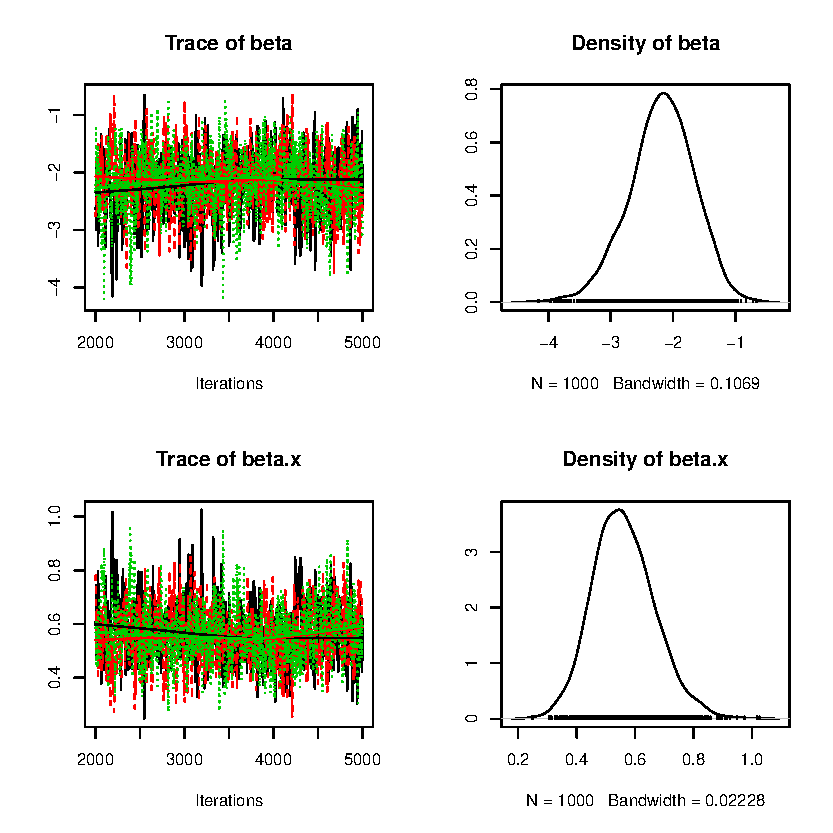
\includegraphics[bb=0 0 400 400, clip, width=300 bp]{example2_jags_results.pdf}
	\end{center}
	\caption{\textsf{coda}クラスオブジェクトのplot出力(JAGS)}
	\label{plot_coda}
\end{figure}
\noindent
各パラメーターについて,各chainの軌跡と,全chainをまとめた事後分布の密度が図示される。

\texttt{gelman.diag()}関数でGelman-Rubin統計量を表示させてみると,
両パラメーターについて1に近い値となっており,
図\ref{plot_coda}の軌跡とあわせて,うまく収束したことが
確認できる。
\begin{lstlisting}
> gelman.diag(post.samp)
Potential scale reduction factors:

       Point est. Upper C.I.
beta            1       1.01
beta.x          1       1.00

Multivariate psrf

1
\end{lstlisting}

%ページ調整
\vspace{2zw}

結果の要約を表示する。
\begin{lstlisting}
> summary(post.samp)

Iterations = 2003:5000
Thinning interval = 3 
Number of chains = 3 
Sample size per chain = 1000 

1. Empirical mean and standard deviation for each variable,
   plus standard error of the mean:

          Mean     SD Naive SE Time-series SE
beta   -2.1827 0.5204 0.009501       0.020194
beta.x  0.5618 0.1067 0.001948       0.004253

2. Quantiles for each variable:

          2.5%     25%     50%     75%  97.5%
beta   -3.2779 -2.4999 -2.1626 -1.8296 -1.243
beta.x  0.3663  0.4891  0.5548  0.6288  0.793

\end{lstlisting}

\noindent
\texttt{beta}の平均値が-2.18,95\%ベイズ信用区間が-3.28〜-1.24,
\texttt{beta.x}の平均値が0.56,95\%ベイズ信用区間が0.37〜0.79
であることがわかる。

%ページ調整
%\vspace{1zw}

つづいて,$\bm{X}$と$\bm{Y}$とのプロットに,$\bm{Y}$の期待値を重ねて表示させてみよう。
\begin{lstlisting}
> beta <- unlist(post.samp[, "beta"])
> beta.x <- unlist(post.samp[, "beta.x"])
> 
> new.x <- seq(0, 10, len = 100)
> logit.p <- beta + beta.x %o% new.x
> exp.y <- k * exp(logit.p) / (1 + exp(logit.p))
> y.mean <- apply(exp.y, 2, mean)
> y.975 <- apply(exp.y, 2, quantile, probs = 0.975)
> y.025 <- apply(exp.y, 2, quantile, probs = 0.025)
> y.995 <- apply(exp.y, 2, quantile, probs = 0.995)
> y.005 <- apply(exp.y, 2, quantile, probs = 0.005)
> 
> plot(x, y, type = "p", ylim = c(0, 10), las = 1)
> lines(new.x, y.mean, lty = 1)
> lines(new.x, y.975, lty = 2)
> lines(new.x, y.025, lty = 2)
> lines(new.x, y.995, lty = 3)
> lines(new.x, y.005, lty = 3)
> legend("bottomright",
+        legend = c("mean", "95% interval", "99% interval"),
+        lty = c(1, 2, 3))
\end{lstlisting}
\noindent
\texttt{post.samp}には,各chainをリストの要素として,
各パラメーターについて
サンプリングされた値が格納されているので,それを取り出して使っている。
1行目と2行目の\texttt{unlist()}関数は,リスト構造になっているものを
まとめて単純なベクトルとする関数である。

Xの値をすこしづつ変えながら,MCMCでサンプリングされたすべての値についてYの値を
計算して,その期待値および信用区間を計算させている。
表示結果は図\ref{example2exp_plot}。
\begin{figure}[htbp]
  \begin{center}
    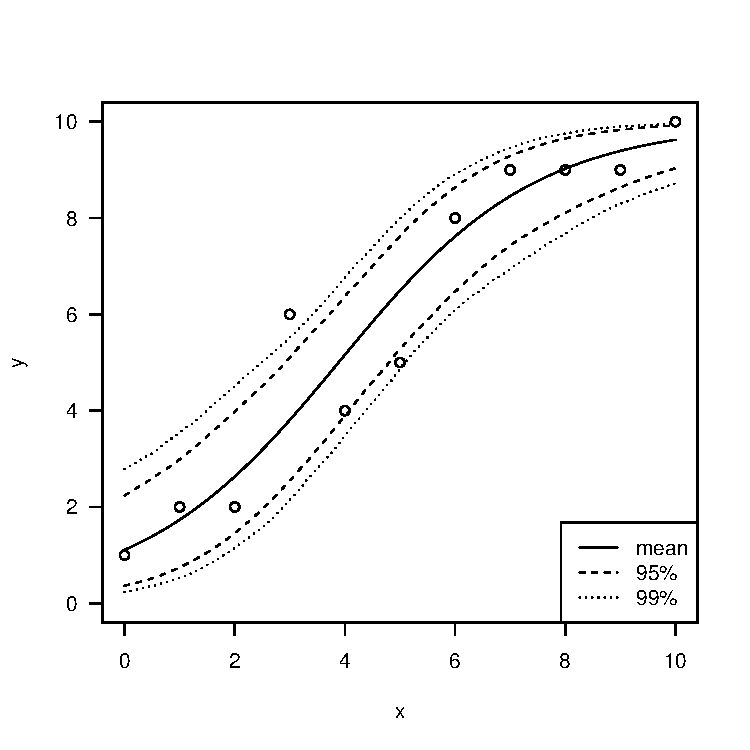
\includegraphics[bb=0 0 360 360, clip, width=240 bp]{example2_exp.pdf}
  \end{center}
  \caption{\ref{logistic}で使用したデータ(点)とYの期待値および信用区間(曲線)}
  \label{example2exp_plot}
\end{figure}

%ページ調整
\pagebreak

\subsubsection{Stanによる例}
同じ問題を\textsf{Stan}により解いてみる。
\textsf{R}スクリプトは\texttt{example2\_Stan.R}である。

RStanを使用する。
\begin{lstlisting}
> library(rstan)
\end{lstlisting}

モデルの定義。\texttt{example2\_code}という文字列にモデルを格納している。
\begin{lstlisting}
> example2_code <- "
+ data {
+   int<lower=0> N;
+   int<lower=0> K;
+   int<lower=0> X[N];
+   int<lower=0> Y[N];
+ }
+ parameters {
+   real beta;
+   real beta_x;
+ }
+ transformed parameters {
+   real<lower=0,upper=1> p[N];
+ 
+   for (i in 1:N) {
+     p[i] <- inv_logit(beta + beta_x * X[i]);
+   }
+ }
+ model {
+   Y ~ binomial(K, p);
+   
+   # priors
+   beta ~ normal(0.0, 1.0e+3);
+   beta_x ~ normal(0.0, 1.0e+3);
+ }
+ "
\end{lstlisting}
\noindent
Stanのモデルの記述は,\texttt{data},\texttt{parameters},
\texttt{transformed parameters},\texttt{model}などのブロックからなる
(詳細はマニュアルを参照)。
また,データや推定するパラメーターには型の宣言が必要である。この際,
とりうる値の上限・下限を設定することもできる。
なお,変数名などに``\texttt{.}''(ピリオド)は使用できない。
かわりに``\texttt{\_}''(アンダーバー)を使うようにする。
また,行末には必ずセミコロン(;)をつける。

chainの数,初期値,保存するパラメーターを設定する。
\begin{lstlisting}
> n.chains <- 3
> inits <- vector("list", 3)
> inits[[1]] <- list(beta = -10, beta_x = 0)
> inits[[2]] <- list(beta =  -5, beta_x = 2)
> inits[[3]] <- list(beta =   0, beta_x = -2)
> pars <- c("beta", "beta_x")
\end{lstlisting}
\texttt{stan()}関数によりStanを実行して,結果を\texttt{fit}というオブジェクトに格納する。
\begin{lstlisting}
> fit <- stan(model_code = example2_code,
+             data = list(X = x, Y = y, N = n, K = k),
+             pars = pars, init = inits, seed = 123,
+             chains = n.chains,
+             iter = 2500, warmup = 500, thin = 2)
\end{lstlisting}
\noindent
\texttt{warmup}はburn-inとおなじものと思ってよい(細かな相違点は参考文献\cite{BDA3}を参照)。

結果を表示する。
\begin{lstlisting}[basicstyle=\ttfamily\footnotesize]
> print(fit)
Inference for Stan model: 404659b08b951f11fe4269ab8d08c9ec.
3 chains, each with iter=2500; warmup=500; thin=2; 
post-warmup draws per chain=1000, total post-warmup draws=3000.

         mean se_mean   sd   2.5%    25%    50%    75%  97.5% n_eff Rhat
beta    -2.19    0.01 0.49  -3.18  -2.52  -2.18  -1.84  -1.29  1581    1
beta_x   0.56    0.00 0.10   0.37   0.49   0.56   0.63   0.76  1553    1
lp__   -51.88    0.02 0.94 -54.30 -52.27 -51.58 -51.19 -50.93  1683    1

Samples were drawn using NUTS(diag_e) at Wed Oct  7 14:10:18 2015.
For each parameter, n_eff is a crude measure of effective sample size,
and Rhat is the potential scale reduction factor on split chains (at 
convergence, Rhat=1).
\end{lstlisting}
\noindent
なお,\texttt{lp\_\_}は対数事後密度である。

\subsubsection{うまくいかないとき}
MCMC計算がうまくいかないときは,まず \textsf{R}コードおよびモデルコード,初期値,データ
をよく見直そう。

\paragraph{エラーになるとき}
エラーが発生してMCMC計算が途中で(あるいは最初から)止まってしまうときは,
まずはエラーメッセージを確認してみる。
とくに\textsf{WinBUGS}や\textsf{OpenBUGS}では,
どこでエラーになっているのか わかりづらいこともままあるが,
下のような点を確認してみる。
\begin{itemize}
\item 構文に誤りはないか? 
\begin{itemize}
\item ``\texttt{\textasciitilde}''と``\texttt{<-}''とを間違えていないか?
\item カッコ(``\texttt{()}''や``\texttt{\{\}}'')の対応はあっているか?
\end{itemize}
\item 変数名などにtypoがないか?
\item 配列の次数や,添字の範囲は正しいか?
\item 初期値がおかしくないか?
\begin{itemize}
\item 例: ガンマ分布なのに負の値を与えている。
\item 数値的にあり得ない値というわけでなくても,あまり極端な値だとエラーが発生することがある。
\end{itemize}
\item モデルに誤りがないか?
\begin{itemize}
\item 事前分布の定義漏れはないか。また逆に,2重定義はされていないか。
\item 確率分布の引数に与える値は,その確率分布にあっているか。
\begin{itemize}
\item 例: ポアソン分布の平均として与える値に負の値が発生している。
\end{itemize}
\end{itemize}
\end{itemize}

\paragraph{MCMC計算が収束しないとき}
エラーは発生しないものの,MCMC計算が収束しないときは下のような点に気をつけてみる。
\begin{itemize}
\item モデルを見直す。
\begin{itemize}
\item データと確率分布があっているか?
\item モデルが必要以上に複雑でないか?
\item 余分なパラメーターがないか?
\end{itemize}
\item Markov chainの長さを長くして,サンプリング間隔を長くする。
  ただし必然的に計算時間は長くなる。モデルの改良のような本質的な
  改善ではないが,もう少し収束をよくしたいというようなときには
  有効なこともある。
\end{itemize}

%ページ調整
%\pagebreak

\subsection{線形混合モデルに相当するモデル,あるいは階層ベイズモデル}
\label{mixed_model}

以下の問題を考える。
\vspace{1zw}

\hspace{18mm}
\begin{minipage}{100mm}
\begin{breakbox}
\noindent
ある調査を,全体を8つのブロックに分けておこない,
各ブロックごとに5組の観察データを
3つの変量($X_1,$ $X_2$, $Y$)について集めた。
変量$Y$は,$X_1$と$X_2$とに影響を受けており,その関係は線形であるとする。
これをモデル化して,パラメーターの推定をおこなう。
このとき,回帰したときの切片にブロックごとに多少の上下(ランダム効果,
あるいは変量効果)があることを想定する。
\end{breakbox}
\end{minipage}

\vspace{1zw}

\paragraph{データ}
今回のデータはあらかじめファイルに保存してある。``\texttt{example3.csv}''から読み込む。
\begin{lstlisting}
> data <- read.csv("example3.csv")
\end{lstlisting}


最初の10行の内容を表示してみると,以下のとおり。
%\vspace{0.5em}
\begin{lstlisting}
> head(data, 10)
   block   x1   x2    y
1      1 5.56 1.64 5.13
2      1 5.13 2.40 4.53
3      1 4.89 3.83 4.37
4      1 5.61 3.92 4.18
5      1 5.01 4.59 2.80
6      2 4.72 3.51 3.14
7      2 4.86 3.13 1.87
8      2 5.86 5.30 4.67
9      2 4.97 3.14 3.60
10     2 4.26 3.29 1.73
\end{lstlisting}

散布図行列を表示して,データを確認する。結果は図\ref{example3_pairs_plot}。

%\vspace{0.5em}
\begin{lstlisting}
> pairs(data)
\end{lstlisting}
%\vspace{0.5em}

\begin{figure}[htbp]
	\begin{center}
		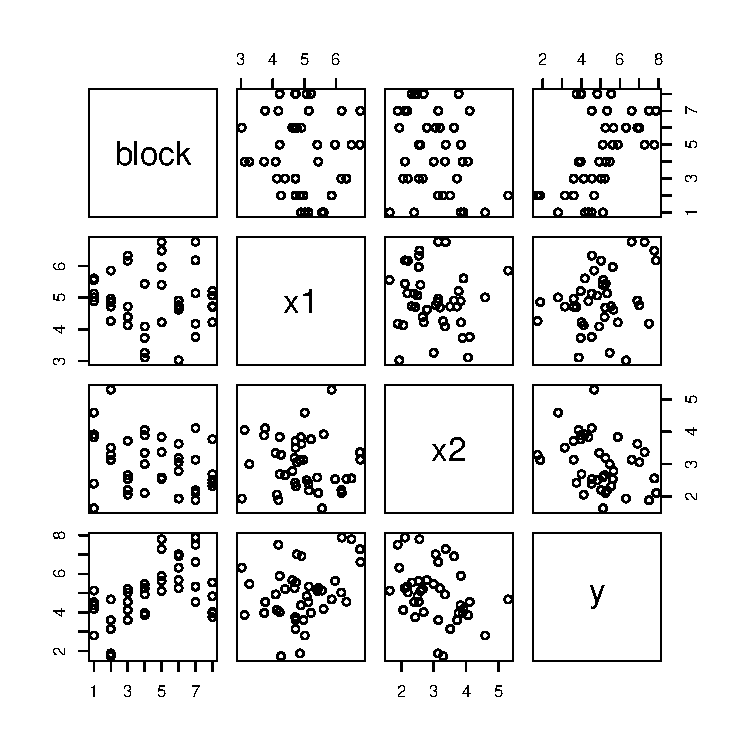
\includegraphics[bb=0 0 360 360, clip, width=270 bp]{example3_pairs.pdf}
	\end{center}
	\caption{\ref{mixed_model}で使用するデータ}
	\label{example3_pairs_plot}
\end{figure}

\textsf{JAGS}を使用してパラメーター推定をおこなうこととする。
使用する\textsf{R}スクリプトは``\texttt{example3.R}''である。

%ページ調整
%\vspace{3zw}

まず,データを行列の形に変換する(BUGSのモデルで使用する形式にあわせるため)。
各行が,各ブロックのデータとなる。

\begin{lstlisting}
> n.block <- max(data$block)      # number of blocks
> n.data <- nrow(data) / n.block  # number of data in a block
>
> x1 <- t(matrix(data$x1, nrow = n.data, ncol = n.block))
> x2 <- t(matrix(data$x2, nrow = n.data, ncol = n.block))
> y  <- t(matrix(data$y,  nrow = n.data, ncol = n.block))
\end{lstlisting}


\texttt{x1}の内容を確認する。
\begin{lstlisting}
> print(x1)
     [,1] [,2] [,3] [,4] [,5]
[1,] 5.56 5.13 4.89 5.61 5.01
[2,] 4.72 4.86 5.86 4.97 4.26
[3,] 4.13 4.72 4.39 6.33 6.17
[4,] 5.44 3.26 3.73 3.11 4.09
[5,] 5.41 6.49 6.76 5.97 4.22
[6,] 3.02 4.76 4.91 4.69 4.62
[7,] 6.77 3.76 4.18 5.14 6.18
[8,] 4.73 4.71 5.07 5.21 4.22
\end{lstlisting}

\paragraph{モデル}
ブロックをランダム効果としてモデルに組み込む。
$\epsilon_{\mathrm{B}i}$をブロック$i$のランダム効果の値とし,
$\sigma_\mathrm{B}$をその事前分布の標準偏差とする。
\begin{align*}
Y_{ij} &\sim \mathrm{Normal}(\mu_{ij}, \sigma^{2}) \\
\mu_{ij} &= \beta + \beta_{1} X_{1ij} + \beta_{2} X_{2ij} + \epsilon_{\mathrm{B}i} \\
\epsilon_{\mathrm{B}i} &\sim \mathrm{Normal}(0, \sigma_\mathrm{B}^{2})
\end{align*}
\noindent
ここで,$\mu_{ij}$はブロック$i$の$j$番目の観測値の期待値,$\sigma$はその標準偏差である。
$\beta$は線形モデル部分の切片,$\beta_{1}$,$\beta_{2}$はそれぞれ$X_{1}$,$X_{2}$の
係数である。

このモデルをBUGS言語で記述すると以下のようになる。
このモデルを,``\texttt{example3\_model.txt}''というファイル名で保存しておく。

\begin{lstlisting}
var
  M,                    # Number of blocks
  N,                    # Number of observations
  X1[N], X2[N],         # Data
  Y[N],
  B[N],                 # Block
  e.B[M],               # Random effect
  beta, beta.1, beta.2, # Parameters
  tau, sigma,
  tau.B, sigma.B;       # Hyperparameters

model {
  for (i in 1:N) {
    Y[i] ~ dnorm(mu[i], tau)
    mu[i] <- beta + beta.1 * X1[i] +
                    beta.2 * X2[i] + e.B[B[i]]
  }
  for (i in 1:M) {
    e.B[i] ~ dnorm(0, tau.B)
  }

  ## Priors
  beta ~ dnorm(0, 1.0E-6)
  beta.1 ~ dnorm(0, 1.0E-6)
  beta.2 ~ dnorm(0, 1.0E-6)
  tau <- 1 / (sigma * sigma)
  tau.B <- 1 / (sigma.B * sigma.B)
  sigma ~ dunif(0, 1.0E+4)
  sigma.B ~ dunif(0, 1.0E+4)
}
\end{lstlisting}

BUGS言語では,変数宣言は必ずしも必要ではないが,高次元配列については
変数宣言が必要となる場合がある。
その場合も,通常のパラメーターの変数などは宣言しなくてもよいが,宣言して
おいたほうがコードの可読性がよくなる(と思う)ので今回は
宣言してある。

このモデルでは,
ブロックによるランダム効果\texttt{e.B[]}の事前分布は,平均が0,分散が1/\texttt{tau.B}
($\texttt{tau.B}=1/\texttt{sigma.B}^{2}$)の
正規分布としている(18行目)。
また,\texttt{sigma.B}の事前分布は[0, 10000]の一様分布としている(28行目)。
すなわちここでは,\texttt{tau.B}(\texttt{sigma.B})が,
パラメーター\texttt{e.B[]}の事前分布を決める
超パラメーター(hyperparameter)となっている(図\ref{example3_schema})。
このようにパラメーターが階層化されているモデルを「階層ベイズモデル」と呼ぶ。

\begin{figure}[htbp]
	\begin{center}
		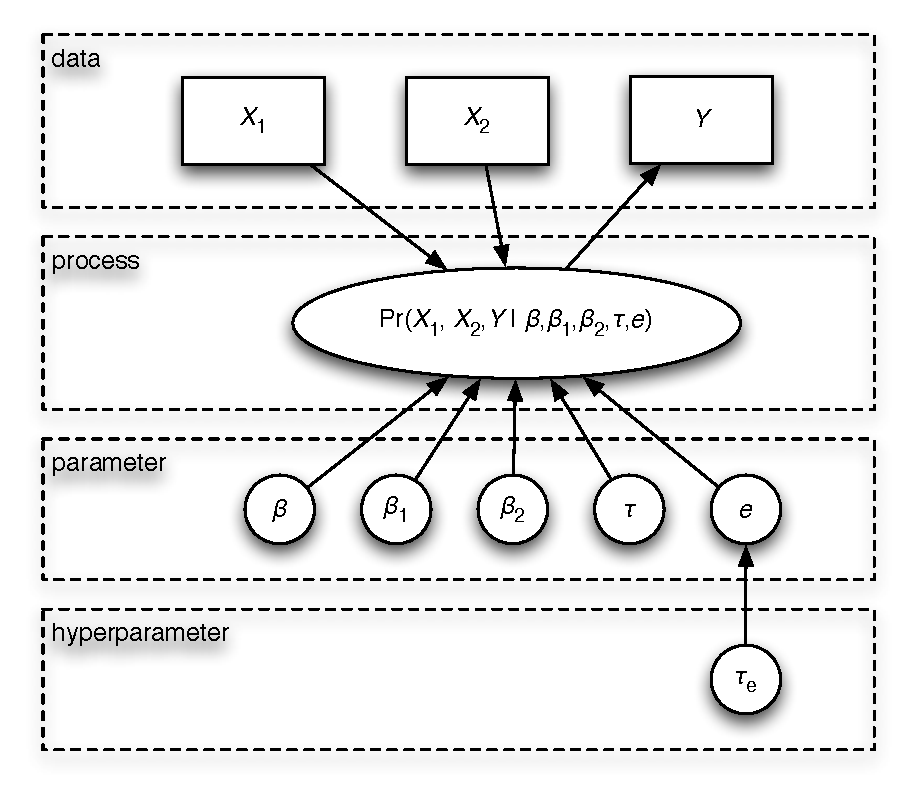
\includegraphics[bb=0 0 440 384, clip, width=320 bp]{example3_schema.pdf}
	\end{center}
	\caption{モデルの概念図}
	\label{example3_schema}
\end{figure}

%ページ調整
%\pagebreak

\paragraph{実行}

前の節と同様に,\textsf{rjags}を使って実行する。
このモデルの場合,\textsf{JAGS}の\texttt{bugs}モジュールを読み込んでおくと
収束が速い(2行目)。

\begin{lstlisting}
> library(rjags)
> load.module("glm")
>
> ## Model file
> model.file <- "example3_model.txt"
> 
> ## Number of chains
> n.chains <- 3
> 
> ## Initial values
> inits <- vector("list", n.chains)
> inits[[1]] <- list(beta =  5, beta.1 = 0, beta.2 = 0,
+                    sigma = 1, sigma.B = 1,
+                    .RNG.seed = 123,
+                    .RNG.name = "base::Mersenne-Twister")
> inits[[2]] <- list(beta =  -5, beta.1 = 10,  beta.2 = 10,
+                    sigma = 10, sigma.B = 10,
+                    .RNG.seed = 1234,
+                    .RNG.name = "base::Mersenne-Twister")
> inits[[3]] <- list(beta = 0, beta.1 = -10,  beta.2 = -10,
+                    sigma = 5, sigma.B = 5,
+                    .RNG.seed = 12345,
+                    .RNG.name = "base::Mersenne-Twister")
> 
> ## Parameters
> pars <- c("beta", "beta.1", "beta.2",
+           "sigma", "sigma.B", "e.B")
> 
> ## MCMC
> model <- jags.model(file = model.file,
+                     data = list(M = n.block, N = n.data,
+                                 X1 = x1, X2 = x2, Y = y),
+                     inits = inits, n.chains = n.chains,
+                     n.adapt = 1000)
  |++++++++++++++++++++++++++++++++++++++++++++++++++| 100%
>
> ## Burn-in
> update(model, n.iter = 1000)
  |**************************************************| 100%
> 
> ## Sampling
> post.samp <- coda.samples(model, n.iter = 5000, thin = 5,
+                           variable.names = pars)
  |**************************************************| 100%
\end{lstlisting}

\paragraph{結果}

結果は以下のようになる。

\begin{lstlisting}
> gelman.diag(post.samp)
Potential scale reduction factors:

        Point est. Upper C.I.
beta         1.000      1.001
beta.1       0.999      1.000
beta.2       1.001      1.004
e.B[1]       1.001      1.002
e.B[2]       1.001      1.001
e.B[3]       1.000      1.001
e.B[4]       0.999      0.999
e.B[5]       1.001      1.003
e.B[6]       1.001      1.003
e.B[7]       1.002      1.005
e.B[8]       1.000      1.000
sigma        1.000      1.002
sigma.B      1.000      1.001

Multivariate psrf

1
> summary(post.samp)

Iterations = 2005:7000
Thinning interval = 5 
Number of chains = 3 
Sample size per chain = 1000 

1. Empirical mean and standard deviation for each variable,
   plus standard error of the mean:

           Mean     SD Naive SE Time-series SE
beta     3.6431 1.2561 0.022934       0.023453
beta.1   0.4762 0.1859 0.003394       0.003395
beta.2  -0.3376 0.1989 0.003631       0.003995
e.B[1]  -0.7389 0.6441 0.011760       0.011762
e.B[2]  -1.5472 0.6489 0.011847       0.010824
e.B[3]  -0.6236 0.6332 0.011560       0.011173
e.B[4]   0.2604 0.6515 0.011894       0.012082
e.B[5]   0.8410 0.6469 0.011810       0.011813
e.B[6]   1.3045 0.6537 0.011935       0.011938
e.B[7]   1.0174 0.6325 0.011549       0.010129
e.B[8]  -0.5042 0.6292 0.011487       0.012747
sigma    0.9169 0.1255 0.002290       0.002414
sigma.B  1.3394 0.5232 0.009553       0.010742

2. Quantiles for each variable:

            2.5%     25%     50%     75%   97.5%
beta     1.24221  2.7958  3.6471  4.4610  6.1945
beta.1   0.12397  0.3545  0.4765  0.5953  0.8445
beta.2  -0.74081 -0.4672 -0.3382 -0.2077  0.0461
e.B[1]  -2.00738 -1.1424 -0.7286 -0.3214  0.4525
e.B[2]  -2.87026 -1.9365 -1.5203 -1.1364 -0.3076
e.B[3]  -1.91307 -1.0123 -0.6190 -0.2163  0.5828
e.B[4]  -1.01832 -0.1383  0.2595  0.6578  1.5216
e.B[5]  -0.40669  0.4229  0.8299  1.2526  2.1243
e.B[6]   0.01952  0.8781  1.2820  1.7131  2.6801
e.B[7]  -0.22065  0.6113  1.0096  1.4158  2.2682
e.B[8]  -1.75477 -0.8872 -0.4968 -0.1091  0.7193
sigma    0.70526  0.8270  0.9071  0.9948  1.1820
sigma.B  0.64972  0.9875  1.2278  1.5691  2.6559

\end{lstlisting}

\texttt{e.B[]}の事後分布は図\ref{example3_e_plot}のようになっている。

%%\begin{breakbox}
%\begin{verbatim}
%plot(NULL, type = "n",
%     xlim = c(-2, 2), ylim = c(0, 2.5),
%     xlab = "value", ylab = "density",
%     main = "Posterior destribution of e[]",
%     las = 1)
%for (i in 1:n.block) {
%  lines(density(post.samp$sims.list$e[,i]), col = i)
%}
%\end{verbatim}
%\end{breakbox}

\begin{figure}[htbp]
	\begin{center}
		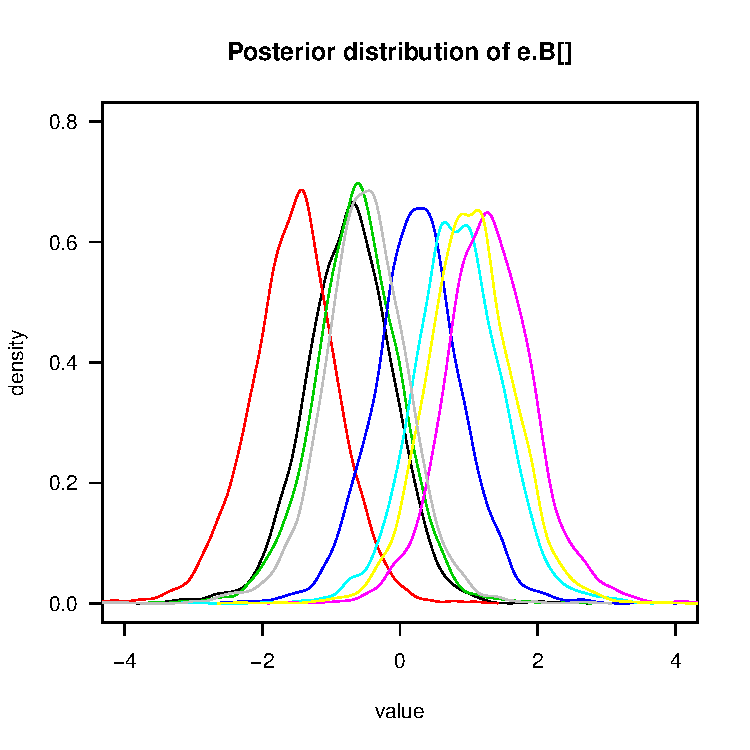
\includegraphics[bb=0 0 360 360, clip, width=270 bp]{example3_e.pdf}
	\end{center}
	\caption{\texttt{e.B[]}の事後分布}
	\label{example3_e_plot}
\end{figure}

%ページ調整
%\pagebreak

\subsubsection*{Nested Indexing}
上の例では2次元配列を使用しているが,配列のインデックスに配列を使用
するNested Indexingという方法もあるので,その例も紹介する。
%データファイルは同じく``\texttt{example3.csv}''だが,
 %\textsf{R}スクリプトは``\texttt{example3-1.R}'',
BUGS言語によるモデルは``\texttt{example3-1\_model.txt}''である。

\paragraph{データ}

まずデータを読み込む。このとき,
データを行列にはせず,ベクトルのままとする。
\begin{lstlisting}
> data <- read.csv("example3.csv")
> n.block <- 8           # number of blocks
> n.row <- nrow(data)    # number of observations
\end{lstlisting}

\texttt{data\$block}にどのブロックのデータであるかが格納されている。
\begin{lstlisting}
> data$block
 [1] 1 1 1 1 1 2 2 2 2 2 3 3 3 3 3 4 4 4 4 4 5 5 5 5 5 6
[27] 6 6 6 6 7 7 7 7 7 8 8 8 8 8
\end{lstlisting}

\paragraph{モデル}

モデルは以下のようになる。\texttt{X1},\texttt{X2},\texttt{Y}が1次元配列に
なっているところ(4〜5行目),\texttt{B}という変数が導入されているところ(6行目),
\texttt{e.B}のインデキシングが\texttt{B}を間に挟んでいるところ(16行目)などが
前のモデルと異なっている。

\begin{lstlisting}
var
  M,                    # Number of blocks
  N,                    # Number of observations
  X1[N], X2[N],         # Data
  Y[N],
  B[N],                 # Block
  e.B[M],               # Random effect
  beta, beta.1, beta.2, # Parameters
  tau, sigma,
  tau.B, sigma.B;       # Hyperparameters

model {
  for (i in 1:N) {
    Y[i] ~ dnorm(mu[i], tau)
    mu[i] <- beta + beta.1 * X1[i] +
                    beta.2 * X2[i] + e.B[B[i]]
  }
  for (i in 1:M) {
    e.B[i] ~ dnorm(0, tau.B)
  }

  ## Priors
  beta ~ dnorm(0, 1.0E-6)
  beta.1 ~ dnorm(0, 1.0E-6)
  beta.2 ~ dnorm(0, 1.0E-6)
  tau <- 1 / (sigma * sigma)
  tau.B <- 1 / (sigma.B * sigma.B)
  sigma ~ dunif(0, 1.0E+4)
  sigma.B ~ dunif(0, 1.0E+4)
}
\end{lstlisting}

\paragraph{実行}

\texttt{jags.model()}関数の\texttt{data}引数は以下のようにする。
\begin{lstlisting}
model <- jags.model(file = model.file,
                    data = list(M = n.block, N = n.data,
                                X1 = data$x1, X2 = data$x2,
                                Y = data$y, B = data$block),
                    inits = inits, n.chains = n.chains,
                    n.adapt = 1000)
\end{lstlisting}

この方法は,前のモデリング方法とは異なり,ブロックごとにデータの数が違うときにも使える。

\subsubsection*{中央化(centering)}

モデル中の説明変数には,それぞれの平均を引いた値をかわりに使用(centering)した
方がマルコフ連鎖の自己相関が小さくなる(参考文献\cite{McCarthy}のBox 5.8)。
たとえば前のモデルなら,15行目の\texttt{beta.1 * X1[i]}を
\texttt{beta.1 * (X1[i] - X1.bar)}とする(\texttt{X1.bar}は\texttt{X1}の平均)。

ただし,\textsf{JAGS}で\texttt{glm}モジュールを使用した場合にはこの技法は不要である
(JAGS User's Manual\cite{JAGS} 4.6節)。

%これを使用した例を以下にしめす。
% \textsf{R}スクリプトは``\texttt{example3-2.R}'',
%BUGSによるモデルは``\texttt{example3-2\_model.txt}''である。
%下のモデルでは,\texttt{X1[]}の平均を\texttt{X1.bar}と,\texttt{X2[]}の平均を\texttt{X2.bar}と
%それぞれ定義し,\texttt{dnorm()}に与える引数\texttt{mu[]}の計算には,
%平均を引いた値を与えるようにしている。

%ページ調整
%\vspace{2zw}
%
%\begin{lstlisting}
%  for (i in 1:N) {
%    Y[i] ~ dnorm(mu[i], tau);
%    mu[i] <- beta + beta.1 * (X1[i] - X1.bar) +
%                    beta.2 * (X2[i] - X2.bar) + e[B[i]];
%  }
%  for (j in 1:M) {
%    e[j] ~ dnorm(0, tau.e);
%  }
%
%  ## centering
%  X1.bar <- mean(X1[]);
%  X2.bar <- mean(X2[]);
%  beta.bar <- beta - beta.1 * X1.bar - beta.2 * X2.bar;
%\end{lstlisting}
%\noindent
%ただしこの場合,求められたパラメーターから予測値を計算する場合
%には,\texttt{beta}の値を補正する必要があることに注意。
%上の例では\texttt{beta.bar}として補正された値を計算している。
%また,交互作用項があるときには結果が変わることがある。
%\footnote{http://hosho.ees.hokudai.ac.jp/{\textasciitilde}kubo/ce/BayesianFrog.html\#toc5}。

%%
%% Zero-Inflated Poissonモデル
%%
\subsection{ゼロ過剰ポアソンモデル}
\label{path}

最後の例題として,実際のデータを解析してみる。

\paragraph{データ}
このデータは,銀閣寺山国有林(京都市左京区)において,クロバイという木の芽生えの数を調べたものである。
調査したのは2002年で,1m×1mの大きさの方形区36か所について,その中で発芽してきた芽生えの数を数えた。
また,各方形区において全天写真を撮影し,それをもとに林冠開空率を求めた。
芽生えの数と林冠開空率との間に関連性があるかどうかを検討する。

データは``\texttt{example4.csv}''というファイルに入っている。
\begin{lstlisting}
"Plot","Num","Light"
1,0,2.680
2,0,1.030
3,3,1.899
   :
36,1,0.412
\end{lstlisting}
\noindent
\texttt{Plot}は方形区番号,\texttt{Num}は芽生えの数,\texttt{Light}は林冠開空率(\%)である。
開空率と芽生えの発生数とをプロットしてみると,図\ref{example4_scatter}のようになる。

\begin{figure}[hbtp]
  \begin{center}
    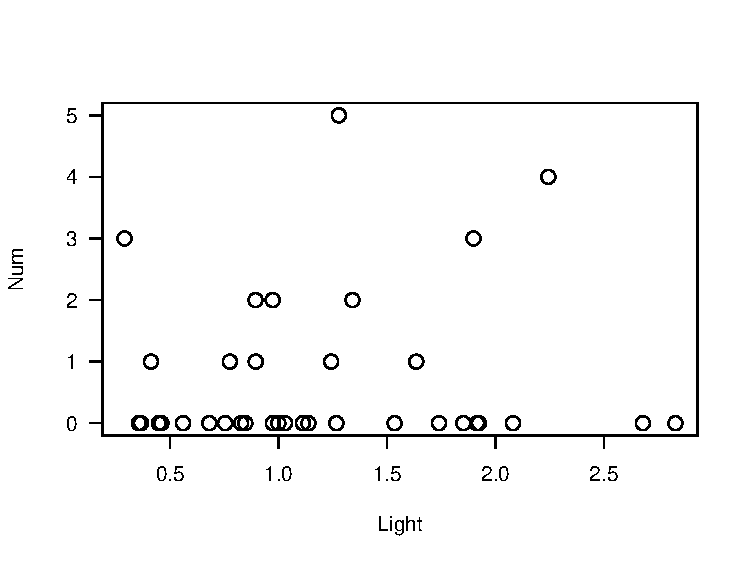
\includegraphics[bb=0 0 360 270, clip, width=300 bp]{example4_scatter.pdf}
  \end{center}
  \caption{開空率と芽生えの発生数との関係}
  \label{example4_scatter}
\end{figure}

単純に,誤差構造をポアソン分布(リンク関数をlog)とした一般化線形モデル(GLM)を適用すると,
以下のような結果となる。

\begin{lstlisting}
> summary(glm(Num ~ Light, family = poisson, data = data))

Call:
glm(formula = Num ~ Light, family = poisson, data = data)

Deviance Residuals: 
    Min       1Q   Median       3Q      Max  
-1.3831  -1.1942  -1.1473   0.3681   3.2771  

Coefficients:
            Estimate Std. Error z value Pr(>|z|)
(Intercept)  -0.5453     0.4234  -1.288    0.198
Light         0.1769     0.2929   0.604    0.546

(Dispersion parameter for poisson family taken to be 1)

    Null deviance: 65.608  on 35  degrees of freedom
Residual deviance: 65.252  on 34  degrees of freedom
AIC: 99.823

Number of Fisher Scoring iterations: 6
\end{lstlisting}

残差逸脱度(Residual deviance)の値が自由度(degree of freedom)の2倍以上となっている。
これは,過分散(overdispersion)が発生していることを示唆している。

もう一度,データをよくみてみると,芽生えの数に0が多いことがわかる(図\ref{example4_barplot})。
このような状態はゼロ過剰(Zero-inflated)と呼ばれる。
こうしたデータを扱うためには,ポアソン分布からはずれて0が多いことを,
そもそも存在する可能性がない場合があると考えて
モデル化する。
このようなモデルはゼロ過剰ポアソンモデル(Zero-Inflated Poisson model; ZIP model)と呼ばれる。

\begin{figure}[hbtp]
  \begin{center}
    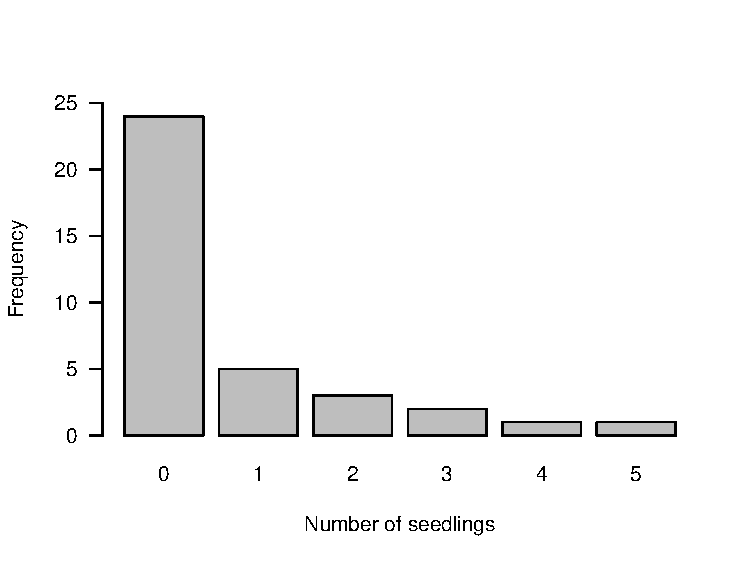
\includegraphics[bb=0 0 360 270, clip, width=300 bp]{example4_barplot.pdf}
  \end{center}
  \caption{芽生えの発生数の頻度分布}
  \label{example4_barplot}
\end{figure}

%ページ調整
%\vspace{1zw}

\paragraph{モデル}
ZIPモデルを扱うBUGSコードは以下のようになる。

\begin{lstlisting}
var
  N,         # Number of observations
  Y[N],      # Number of new seedlings
  X[N],      # Proportion of open canopy
  lambda[N], # Poisson mean
  z[N],      # 0: absent, 1: at least latently present
  p,         # Probability of the presence (at least latently)
  beta,      # Intercept in the linear model
  beta.x;    # Coefficient of X in the linear model
model {
  for (i in 1:N) {
    Y[i] ~ dpois(lambda[i])
    lambda[i] <- z[i] * exp(beta + beta.x * X[i])
    z[i] ~ dbern(p)
  }
  ## Priors
  p ~ dunif(0, 1)
  beta ~ dnorm(0, 1.0E-4)
  beta.x ~ dnorm(0, 1.0E-4)
}
\end{lstlisting}

%% モデルの説明

芽生えの数が0となるのは以下の2通りであるとしてモデル化している。
\begin{enumerate}
\item 潜在的にも存在しない場合($z=0$)
\item 潜在的には存在する可能性があるが($z=1$)
ポアソン分布にしたがって0となった場合($\mathrm{Poisson}(0|\lambda)$)
\end{enumerate}
そして,$z$が0になるか1になるかは,確率$p$のベルヌーイ分布にしたがうとする。
潜在的には存在する可能性がある場合には,ポアソン分布部分の平均$\lambda$は
$\log\lambda = \beta + \beta_{x}X$であるとする。


\paragraph{結果}
これも同様に\textsf{rjags}を使って計算したところ
(burn-in 2000回,繰り返し回数 10000回,サンプリング間隔 10回),結果は以下のようになった。

\begin{lstlisting}
> summary(post.samp)

Iterations = 2010:12000
Thinning interval = 10 
Number of chains = 3 
Sample size per chain = 1000 

1. Empirical mean and standard deviation for each variable,
   plus standard error of the mean:

           Mean     SD Naive SE Time-series SE
beta   -0.09412 0.5810 0.010607       0.016938
beta.x  0.49827 0.4083 0.007455       0.011882
p       0.43111 0.1037 0.001893       0.001893

2. Quantiles for each variable:

          2.5%     25%      50%    75%  97.5%
beta   -1.2656 -0.4963 -0.07169 0.2823 1.0174
beta.x -0.3225  0.2259  0.50584 0.7898 1.2494
p       0.2468  0.3584  0.42481 0.5002 0.6501

\end{lstlisting}
存在する確率pの事後平均は0.431,95\%信用区間は0.247〜0.650と推定された。
また,線形モデル部分の切片betaおよび開空率の係数beta.xの事後平均はそれぞれ
-0.09および0.498と,95\%信用区間はそれぞれ-1.226〜1.017および-0.323〜1.249
と推定された。開空率の係数の事後平均は,GLMでの推定値0.177よりも大きい値と
なった。

%ページ調整
%\pagebreak

\section{さらに学ぶには}

今回紹介したモデルは,モデルとしては簡単なものである。
実際に研究で使用されるモデルはもっと複雑なものであることが多い。
``Models for Ecological Data''\cite{Clark},
``Hierarchical modelling for the environmental sciences''\cite{Clark_Gelfand},
``Introduction to WinBUGS for ecologists''\cite{IWE},
``Bayesian population analysis using WinBUGS''\cite{BPA},
``Bayesian methods for ccology''\cite{McCarthy}などにて,
生態学・環境科学における実例が紹介されている。

日本語のものでは,
『データ解析のための統計モデリング入門』\cite{Kubo:Modeling}が,
GLM$\rightarrow$GLMM$\rightarrow$階層ベイズモデル
と,順序を追ってわかりやすく説明している。
空間統計モデリングについては,2009年の『日本生態学会誌』において,
久保\cite{Kubo}がその基本を解説して
おり,深澤ほか\cite{Fukasawa_et_al}が実例の紹介をおこなっている。
『マルコフ連鎖モンテカルロ法』\cite{Toyoda}には,
共分散構造分析におけるベイズ推定など,社会科学への応用例がある。
同じ著者の『基礎からのベイズ統計学』\cite{Toyoda2015}も,基本から
Hamiltonian Monte Carlo法のアルゴリズムまで丁寧に解説されている。
また,『岩波データサイエンス Vol.1』\cite{Iwanami_vol1}には,
\textsf{JAGS}や\textsf{Stan}などを用いた解析方法の記事があり,
サポートページ\footnote{\url{https://sites.google.com/site/iwanamidatascience/vol1/support_tokushu}}では,コードや解説動画なども公開されている。


その他,MCMCや階層ベイズモデルについて目に付いたものを参考文献リストに入れて
おいたので,参考にされたい。

%ページ調整
%\pagebreak

%% 参考文献
\begin{thebibliography}{99}
\bibitem{PRML} Bishop C.M. (2006) Pattern recognition and machine learning.
  Springer-Verlag, New York.
  (日本語訳: 元田浩・栗田多喜夫・樋口知之・松本裕治・村田昇監訳 (2012)
  「パターン認識と機械学習 上/下」丸善, 東京)
\bibitem{Handbook} Brooks S., Gelman A., Jones G.L., Meng X.-L. (2011)
Handbook of Markov chain Monte Carlo. Chapman \& Hall/CRC, Boca Raton. 
\bibitem{Clark} Clark J.S. (2007) Models for ecological data.
  Princeton University Press, Princeton.
\bibitem{Clark_Gelfand} Clark J.S., Gelfand A.E. (2006) Hierarchical modelling
  for the environmental sciences. Oxford University Press, New York.
%\bibitem{Fukasawa} 深澤圭太・角谷拓 (2009) 始めよう! ベイズ推定によるデータ解析.
%  日本生態学会誌 59:167--170.\\
%  \texttt{http://ci.nii.ac.jp/naid/110007340208}
\bibitem{Fukasawa_et_al} 深澤圭太・石濱史子・小熊宏之・武田知己・田中信行・
  竹中明夫 (2009) 条件付き自己回帰モデルによる空間自己相関を考慮した生物の分布
  データ解析. 日本生態学会誌 59:171--186. \\
  \url{http://ci.nii.ac.jp/naid/110007340206}
\bibitem{Furutani} 古谷知之 (2008) ベイズ統計データ分析 --- R \& WinBUGS ---.
  朝倉出版, 東京.
\bibitem{BDA3} Gelman A, Carlin J.B., Stern H.S., Dunson D.B., Vehtari A.,
  Rubin D.B. (2014) Bayesian data analysis, 3rd ed.
  Chapman \& Hall/CRC, Boca Raton.
\bibitem{Gilks} Gilks W.R., Richardson S.R., Spiegelhalter D.J. (eds.) (1996)
  Markov chain Monte Carlo in practice. Chapman \& Hall/CRC, Boca Raton.
\bibitem{Iba} 伊庭幸人 (2003) ベイズ統計と統計物理. 岩波書店, 東京.
\bibitem{Iba2005} 伊庭幸人 (2005) マルコフ連鎖モンテカルロ法の基礎. 
  (伊庭幸人・種村正美・大森裕浩・和合肇・佐藤整尚・高橋明彦(著)
  「計算統計II ---マルコフ連鎖モンテカルロ法とその周辺---」
  岩波書店, 東京): 1--106.
\bibitem{Iwanami_vol1} 岩波データサイエンス刊行委員会(編) (2015) 岩波データサイエンス Vol.1.
岩波書店, 東京. \\
シリーズサポートページ \url{https://sites.google.com/site/iwanamidatascience/}
\bibitem{IWE} K\'ery M. (2010) Introduction to WinBUGS for ecologists:
  a Bayesian approach to regression, ANOVA, mixed models and related analyais.
  Academic Press, Waltham.
\bibitem{BPA} K\'ery M, Schaub M. (2011) Bayesian population analysis using WinBUGS.
  Academic Press, Waltham.
\bibitem{DBDA2} Kruschke J. (2014) Doing Bayesian data analysis, 2nd ed.:
  a tutorial with R, JAGS, and Stan. Academic Press, Waltham.
\bibitem{Kubo} 久保拓弥 (2009) 簡単な例題で理解する空間統計モデル. 
  日本生態学会誌 59: 187--196. \\
  \url{http://ci.nii.ac.jp/naid/110007340204}
\bibitem{Kubo:IEICE} 久保拓弥 (2009) 最近のベイズ理論の進展と応用[I]
  階層ベイズモデルの基礎. 電子情報通信学会誌 92:881--885.\\
  \url{http://eprints.lib.hokudai.ac.jp/dspace/handle/2115/39717}
\bibitem{Kubo:Modeling} 久保拓弥 (2012) データ解析のための統計モデリング入門 ---
   一般化線形モデル・階層ベイズモデル・MCMC---. 岩波書店, 東京.
\bibitem{Kyo} 姜興起 (2010) ベイズ統計データ解析. 共立出版, 東京.
\bibitem{Link2012} Link, W.A., Eaton, M.J. (2012) On thinning of chains in MCMC.
Methods in Ecology and Evolution 3: 112--115. doi: 10.1111/j.2041-210X.2011.00131.x
\bibitem{OpenBUGS} Lunn D., Spiegelhalter D., Thomas A., Best N. (2009)
  {The BUGS project: Evolution, critique, and future directions}.
  {Statistics in Medicine} {28}:3049--3067.
\bibitem{BUGSBook} Lunn D., Jackson C, Besk N., Thomas A., Spiegelhalter D.
  (2012) The {BUGS} Book. Chapman \& Hall/CRC, Boca Raton.
\bibitem{MCMCpack} Martin A.D., Quinn, K.M. (2006) Applied Bayesian inference in R
using MCMCpack. R News 6(1):2--7. \\
    \url{http://cran.r-project.org/doc/Rnews/Rnews_2006-1.pdf}
%\bibitem{Martin} Martin J-M, Robert C. P. (2007) Bayesian core: A practical
%  approach to computational Bayesian statistics. Springer, New York.
\bibitem{McCarthy} McCarthy M.A. (2007) Bayesian methods for ecology.
  Cambridge University Press, New York.
  (日本語訳: 野間口眞太郎訳 (2009) 「生態学のためのベイズ法」共立出版, 東京.)
\bibitem{Ntzoufras} Ntzoufras I. (2009) Bayesian modeling using WinBUGS.
  Wiley, Hoboken.
\bibitem{JAGS} Plummer M. (2015) JAGS version 4.0.0 user manual.\\
  \url{http://sourceforge.net/projects/mcmc-jags/}
\bibitem{R} R Core Team (2015)
   R: A Language and Environment for Statistical Computing.
   R Foundation for Statistical Computing, Vienna.\\
   \url{http://www.R-project.org/}
\bibitem{IMCMR} Robert C.P., Casella G. (2010) Introducing Monte Carlo Methods with R.
  Springer, New York.
  (日本語訳: 石田・石田訳 (2012) 「Rによるモンテカルロ法入門」丸善, 東京.)
\bibitem{WinBUGS} Spiegelhalter D., Tomas A., Best N., Lunn D. (2003)
  WinBUGS user manual version 1.4.\\
  \url{http://www.mrc-bsu.cam.ac.uk/bugs/winbugs/manual14.pdf}
\bibitem{Stan} Stan Development Team (2015) Stan Modeling Language:
  User's Guide and Reference Manual, Version 2.7.0.
  \url{http://mc-stan.org/}
\bibitem{Tango} 丹後俊郎 (2000) 統計モデル入門. 朝倉書店, 東京.
\bibitem{Terui} 照井伸彦 (2010) Rによるベイズ統計分析. 朝倉書店, 東京.
\bibitem{BUGS} Thomas A. (2006) The BUGS language.
  R News 6(1): 17--21. \\
  \url{http://cran.r-project.org/doc/Rnews/Rnews_2006-1.pdf}
\bibitem{Thomas} Thomas A., O'Hara B., Ligges U., Sturtz S. (2006) Making BUGS open.
  R News 6(1): 12--17. \\
  \url{http://cran.r-project.org/doc/Rnews/Rnews_2006-1.pdf}
%\bibitem{Tomita} 富田基史・花岡創 (2009) 階層ベイズモデルによる複雑な生態学的
%  プロセスの推定: ブナの花粉散布空間パターン推定を例に.
%  日本生態学会誌 59: 197--206.  \\
%  \texttt{http://ci.nii.ac.jp/naid/110007340202}
\bibitem{Toyoda} 豊田秀樹 (2008) マルコフ連鎖モンテカルロ法. 朝倉書店, 東京.
\bibitem{Toyoda2015} 豊田秀樹(編著) (2015) 基礎からのベイズ統計学
  ---ハミルトニアンモンテカルロ法による実践的入門---. 朝倉書店, 東京.
\bibitem{Wagou} 和合肇 (2005) ベイズ統計学による分析. (牧厚志・和合肇・
  西山茂・人見光太郎・吉川肇子・吉田栄介・濱岡豊(著)「経済・経営のための
  統計学」有斐閣, 東京):243--284.
\bibitem{Watanabe} 渡辺澄夫 (2012) ベイズ統計の理論と方法. コロナ社, 東京.
%\bibitem{Yamamichi} 山道真人・角谷拓 (2009) マルコフ連鎖モンテカルロ(MCMC)法を
%  用いたシミュレーションモデルのパラメータ推定: ベイジアンキャリブレーション入門.
%  日本生態学会誌 59:207--216. \\
%  \texttt{http://ci.nii.ac.jp/naid/110007340200}
\end{thebibliography}


\end{document}
